\documentclass[aspectratio=169,10pt]{beamer}

\usetheme{Madrid}
\usecolortheme{seahorse}
\usefonttheme{professionalfonts}

\usepackage{amsmath,amssymb,amsthm}
\usepackage{mathtools}
\usepackage{listings}
\usepackage{xcolor}
\usepackage{booktabs}
\usepackage{graphicx}
\usepackage{bm}
\usepackage{enumerate}

\graphicspath{{figures/}}

%% Python listing style
\lstdefinestyle{python}{
  language=Python,
  basicstyle=\ttfamily\scriptsize,
  keywordstyle=\color{blue!80!black}\bfseries,
  stringstyle=\color{orange!80!black},
  commentstyle=\color{green!50!black}\itshape,
  numberstyle=\tiny\color{gray},
  numbers=left, stepnumber=1,
  frame=single, breaklines=true,
  showstringspaces=false, tabsize=4,
  backgroundcolor=\color{gray!7},
}

\title[MC Theory -- Ch.4]{Lectures on Monte Carlo Theory}
\subtitle{Chapter 4: Simulation Output Analysis: Independent Replications}
\author{Based on Lorek \& Rolski}
\date{}

\setbeamertemplate{navigation symbols}{}
\setbeamertemplate{footline}[frame number]

\begin{document}

% ------------------------------------------------------------------ title
\begin{frame}
  \titlepage
\end{frame}

% ------------------------------------------------------------------ TOC
\begin{frame}{Chapter Outline}
  \tableofcontents
\end{frame}

\section{Introduction: Why Output Analysis?}
\section{4.1 Estimation of $I = \mathbb{E}Y$}
\section{4.2 Estimation of $k(I)$ -- the Delta Method}
\section{4.3 Estimators of a Quantile}
\section{4.4 More on Absolute vs Relative Errors}
\section{4.5 Conclusions}

%%==================================================================
%% INTRODUCTION
%%==================================================================

\begin{frame}[allowframebreaks]{Introduction: Why Output Analysis?}

When we run a Monte Carlo simulation, every output is a random number.
If we estimate $I = \pi$ by simulating $R = 1{,}000$ random points and
obtain $\hat{I} = 3.14$, that single number tells us very little on its own.
Is it close to the truth?  By how much could it be wrong?

\textbf{Output analysis} gives scientific meaning to simulation results.
Its two central goals are:
\begin{enumerate}
  \item Build a \emph{confidence interval} (CI) that brackets the true $I$
        with a specified probability $1 - \alpha$ (alpha, the significance level),
        for example 95\%.
  \item Decide how many replications $R$ are needed to achieve a desired
        half-width $b$ for that CI.
\end{enumerate}

The mathematical backbone is the \textbf{Central Limit Theorem (CLT)}, which
guarantees that the sample mean is approximately normally distributed for
large $R$, allowing us to use standard normal quantiles to build CIs.

\begin{block}{The Central Goal of Chapter 4}
  Establish the \textbf{fundamental relationship}
  \[
    b = \frac{z_{1-\alpha/2}\,D}{\sqrt{R}},
  \]
  where $b$ is the CI half-width (how precise the estimate is), $R$ is the
  number of replications (how many simulations we run), $z_{1-\alpha/2}$
  (z sub one-minus-alpha-over-two) is the standard normal quantile at level
  $1-\alpha/2$ (for 95\% confidence, $z_{0.975} = 1.96$), and $D$ is the
  variability constant of the particular estimation problem.  Any two of
  these three quantities determine the third.
\end{block}

\framebreak

\begin{block}{General Problem Setup}
  We wish to estimate a quantity expressible as
  \[
    I = \mathbb{E}Y,
  \]
  where $\mathbb{E}$ (blackboard-bold E) denotes expectation (the theoretical
  average), and $Y$ is a random variable we can simulate, satisfying
  $\mathbb{E}Y^2 < \infty$ (finite second moment, i.e.\ finite variance).
  We draw $R$ independent, identically distributed (i.i.d.) copies
  $Y_1, Y_2, \ldots, Y_R$ and form their sample mean $\hat{Y}_R$.
\end{block}

Two fundamentally different notions of error arise throughout:

\textbf{Absolute error:} $|\hat{I} - I|$ measures the raw distance between
the estimate and the truth.  We want this to be at most $\varepsilon$ (epsilon)
with high probability.

\textbf{Relative error:} $|\hat{I}/I - 1| = |\hat{I} - I|/I$ measures the
discrepancy as a fraction of the true value.  It is more informative when $I$
itself is small -- for example, when $I$ is a rare-event probability.

\begin{block}{Error Control Conditions (for $\varepsilon, \delta \in (0,1)$)}
  \begin{align*}
    \text{(E1) Absolute: } & \mathbb{P}(|\hat{I} - I| \geq \varepsilon) \leq \delta \\
    \text{(E2) Relative: } & \mathbb{P}(|\hat{I}/I - 1| \geq \varepsilon) \leq \delta
  \end{align*}
  Here $\delta$ (delta) is the permitted probability of failure (for 99\%
  confidence, $\delta = 0.01$).  Condition (E2) is strictly harder than (E1)
  when $I < 1$: it requires the error to be small \emph{relative} to the
  true value, not just absolutely small.
\end{block}

\begin{alertblock}{Key Takeaway}
  This chapter focuses on absolute error for most of Sections 4.1--4.3, then
  returns to relative error in Section 4.4, where we show it is dramatically
  harder when $I$ is small --- motivating variance reduction techniques.
\end{alertblock}

\end{frame}

%%==================================================================
%% SECTION 4.1.1 -- SAMPLE MEAN
%%==================================================================

\begin{frame}[allowframebreaks]{4.1.1 The Sample Mean Estimator}

We want to compute $I = \mathbb{E}Y$.  The most natural estimator is the
average of $R$ independent simulation runs.

\begin{block}{Sample Mean Estimator (Eq.\ 1.1)}
  \[
    \hat{Y}_R = \frac{1}{R} \sum_{j=1}^{R} Y_j,
  \]
  where $\sum_{j=1}^{R}$ (Sigma, meaning ``sum'') adds up the values from
  $j=1$ to $j=R$.  Here $Y_1, Y_2, \ldots, Y_R$ are i.i.d.\ copies of $Y$,
  each being one independent simulation run, and $R$ (capital R) is the total
  number of replications.
\end{block}

This estimator has two fundamental properties.

\textbf{Unbiasedness.}  Taking expectations of both sides:
$\mathbb{E}\hat{Y}_R = \frac{1}{R}\sum_{j=1}^R \mathbb{E}Y_j = \mathbb{E}Y = I$.
The expected value of the estimate equals the truth, so there is no systematic
over- or under-estimation --- the estimator does not ``lean'' in any direction.

\textbf{Strong consistency.}  By the Strong Law of Large Numbers (SLLN),
$\hat{Y}_R \to I$ with probability 1 as $R \to \infty$.  In plain terms:
if we run infinitely many replications, the average converges to the truth
with certainty.  This implies \emph{weak consistency}: for every fixed $b > 0$,
$\mathbb{P}(|\hat{Y}_R - I| \geq b) \to 0$ as $R \to \infty$.  Weak consistency
in turn implies: for every $b > 0$ and $0 < \alpha < 1$, there exists $R_0$
such that for all $R \geq R_0$:
\[
  \mathbb{P}(\hat{Y}_R - b < I \leq \hat{Y}_R + b) \geq 1 - \alpha. \tag{1.2}
\]
This is the key guarantee: for large enough $R$, the random interval
$(\hat{Y}_R - b,\, \hat{Y}_R + b)$ contains the true value $I$ with high
probability $1-\alpha$.

\framebreak

The guarantee in (1.2) is existential --- it tells us such $R_0$ exists but
not how large it is.  Two tools give quantitative bounds.

\begin{block}{Chebyshev's Inequality-Based Error Bound (Remark~4.1.1)}
  Chebyshev's inequality states: for any random variable $X$ with finite
  variance, $\mathbb{P}(|X - \mathbb{E}X| \geq t) \leq \mathrm{Var}(X)/t^2$,
  for any $t > 0$.  Applying this to $\hat{Y}_R$ (which has variance
  $\sigma_Y^2/R$, where $\sigma_Y^2 = \mathrm{Var}(Y)$ is the variance of
  a single observation) with $t = b_R$:
  \[
    \mathbb{P}(|\hat{Y}_R - I| \geq b_R) \leq \frac{\sigma_Y^2/R}{b_R^2}.
  \]
  Setting this bound equal to $\alpha$ (alpha, the significance level) and
  solving for $b_R$ gives the \emph{Chebyshev half-width}:
  \[
    b_R^{\mathrm{Ch}} = \frac{1}{\alpha^{1/2}} \cdot \frac{\sigma_Y}{\sqrt{R}}. \tag{1.3}
  \]
  Here $\sigma_Y = \sqrt{\mathrm{Var}(Y)}$ (sigma sub Y) is the standard
  deviation of a single observation -- how spread out one simulation output is.
  Note $b_R = O(R^{-1/2})$: the error decreases at the \emph{Monte Carlo rate},
  regardless of the dimension of the problem.
\end{block}

\begin{alertblock}{How to Read the Chebyshev Bound}
  This bound is valid for \emph{any} distribution of $Y$ and any sample size
  $R$ (it is non-asymptotic).  However, it is quite conservative: it ignores
  the shape of the distribution and only uses the variance.  The CLT gives
  a much sharper bound at the cost of holding only approximately for large $R$.
\end{alertblock}

\framebreak

\begin{block}{Central Limit Theorem (CLT, Eq.\ 1.4)}
  Let $Y_1, Y_2, \ldots, Y_R$ be i.i.d.\ with standard deviation
  $\sigma_Y = \sqrt{\mathrm{Var}\,Y} < \infty$.  Define
  $I = \mathbb{E}Y$.  As $R \to \infty$:
  \[
    \mathbb{P}\!\left(\sum_{j=1}^{R} \frac{Y_j - I}{\sigma_Y \sqrt{R}} \leq x\right)
      \;\longrightarrow\; \Phi(x),
  \]
  where $\Phi(x)$ (Phi of x) is the cumulative distribution function (CDF)
  of the standard normal distribution $\mathcal{N}(0,1)$.  Equivalently,
  $\sqrt{R}(\hat{Y}_R - I) \xrightarrow{\mathcal{D}} \mathcal{N}(0, \sigma_Y^2)$
  (converges in distribution to a normal with mean 0 and variance $\sigma_Y^2$).
\end{block}

Let $z_{1-\alpha/2} = \Phi^{-1}(1 - \alpha/2)$ denote the $(1-\alpha/2)$-quantile
of the standard normal.  For $\alpha = 0.05$: $z_{0.975} = 1.96$.
For $\alpha = 0.01$: $z_{0.995} = 2.576$.  From the CLT, rearranging to
isolate $I$:

\begin{block}{The Fundamental Relationship (Eq.\ 1.6)}
  \[
    b = z_{1-\alpha/2} \frac{\sigma_Y}{\sqrt{R}}, \tag{1.6}
  \]
  where $b$ is the CI half-width, $z_{1-\alpha/2}$ is the normal quantile
  (for 95\% CI: $z_{0.975} = 1.96$), $\sigma_Y = \sqrt{\mathrm{Var}(Y)}$
  is the single-observation standard deviation, and $R$ is the number of
  replications.  This relationship says: the half-width shrinks as $1/\sqrt{R}$
  -- doubling accuracy requires \emph{quadrupling} the number of replications.
\end{block}

\begin{block}{Required Number of Replications (Eq.\ 1.7)}
  Solving (1.6) for $R$: to achieve half-width $b$ at confidence level
  $1-\alpha$, we need
  \[
    R = z_{1-\alpha/2}^2 \frac{\sigma_Y^2}{b^2}. \tag{1.7}
  \]
  For 95\% confidence ($\alpha = 0.05$): $R = 1.96^2 \cdot \sigma_Y^2/b^2
  \approx 3.84\,\sigma_Y^2/b^2$.
\end{block}

\framebreak

\begin{exampleblock}{Remark~4.1.5 -- CLT vs.\ Chebyshev: Quantitative Savings}
  The ratio of the CLT half-width to the Chebyshev half-width is:
  \[
    \frac{b^{\mathrm{CLT}}}{b^{\mathrm{Ch}}}
      = \frac{z_{1-\alpha/2}\,\sigma_Y/\sqrt{R}}{\sigma_Y/(\alpha^{1/2}\sqrt{R})}
      = z_{1-\alpha/2}\,\alpha^{1/2}
      = 1.96 \times \sqrt{0.05} = 0.4382 \quad (\alpha = 0.05).
  \]
  Since required sample size $R \propto b^{-2}$, the CLT-based formula needs
  only $(0.4382)^2 \approx 19.2\%$ as many replications as Chebyshev to
  achieve the same nominal confidence level.  That is a roughly $5\times$
  reduction in computational cost.  The price is that the CLT result is
  an approximation valid for large $R$, while Chebyshev is exact for any $R$.
\end{exampleblock}

\begin{alertblock}{Key Insight: The Monte Carlo Rate}
  The error $b \propto R^{-1/2}$ is independent of the dimension $d$ of the
  problem.  This is the crucial advantage of Monte Carlo over deterministic
  integration rules, which suffer a \emph{curse of dimensionality} (error
  growing exponentially in $d$).
\end{alertblock}

\end{frame}

\begin{frame}[allowframebreaks]{4.1.1 Confidence Intervals in Practice}

In practice, $\sigma_Y^2 = \mathrm{Var}(Y)$ is unknown.  We estimate it
from the data using the \textbf{sample variance}.

\begin{block}{Sample Variance (Two Definitions)}
  Given observations $Y_1, \ldots, Y_R$ with sample mean $\hat{Y}_R$:
  \begin{align*}
    \hat{S}_R^2 &= \frac{1}{R-1} \sum_{j=1}^{R} (Y_j - \hat{Y}_R)^2
      \quad \text{(unbiased: $\mathbb{E}\hat{S}_R^2 = \sigma_Y^2$)} \\[4pt]
    \hat{\sigma}_R^2 &= \frac{1}{R} \sum_{j=1}^{R} (Y_j - \hat{Y}_R)^2
      \quad \text{(biased, but simpler)}
  \end{align*}
  In both formulas, $(Y_j - \hat{Y}_R)^2$ is the squared deviation of the
  $j$-th observation from the sample mean.  Summing and dividing gives the
  average squared deviation -- the sample variance.  The divisor $R-1$ in
  $\hat{S}_R^2$ (Bessel's correction) makes it unbiased.  For large $R$,
  both definitions are nearly identical.
\end{block}

Substituting $\hat{S}_R$ for $\sigma_Y$ in (1.6) remains valid asymptotically
by Slutsky's theorem (if $\hat{S}_R \to \sigma_Y$ then ratios behave
normally).  This gives the practical confidence interval:

\begin{block}{$(1-\alpha)$-Confidence Interval (Eq.\ 1.9)}
  \[
    \left(\hat{Y}_R - z_{1-\alpha/2}\frac{\hat{S}_R}{\sqrt{R}},\;\;
           \hat{Y}_R + z_{1-\alpha/2}\frac{\hat{S}_R}{\sqrt{R}}\right). \tag{1.9}
  \]
  This interval is centered at the sample mean $\hat{Y}_R$, with half-width
  $z_{1-\alpha/2}\,\hat{S}_R/\sqrt{R}$.  Here $\hat{S}_R/\sqrt{R}$ is called
  the \emph{standard error of the mean} -- it measures how accurately
  $\hat{Y}_R$ estimates $I$.  For 95\% confidence ($\alpha = 0.05$,
  $z_{0.975} = 1.96$): the CI is $\hat{Y}_R \pm 1.96\,\hat{S}_R/\sqrt{R}$.
\end{block}

\begin{alertblock}{How to Read This Interval}
  The 95\% CI does NOT mean ``there is a 95\% probability that $I$ lies in
  this specific interval.''  Rather, if we repeated this experiment many times,
  95\% of the resulting intervals would contain the true $I$.  Once computed,
  the specific interval either contains $I$ or it does not.
\end{alertblock}

\framebreak

\begin{block}{Online / Recursive Update Formulas (Eqs.\ 1.11--1.12)}
  These allow updating the mean and variance without storing all $R$
  observations.  After each new observation $Y_{R+1}$:
  \begin{align}
    \hat{Y}_{R+1} &= \hat{Y}_R + \frac{Y_{R+1} - \hat{Y}_R}{R+1}, \tag{1.11} \\[4pt]
    \hat{\sigma}_{R+1}^2 &= \hat{\sigma}_R^2 + (\hat{Y}_R)^2 - (\hat{Y}_{R+1})^2
      + \frac{(Y_{R+1})^2 - \hat{\sigma}_R^2 - (\hat{Y}_R)^2}{R+1}. \tag{1.12}
  \end{align}
  Each new observation $Y_{R+1}$ updates both statistics in $O(1)$ time
  and $O(1)$ memory.  This is a streaming (online) algorithm, essential
  for very large simulations where storing all $Y_j$ is impractical.
\end{block}

\textbf{Worked example of recursive update:}
Start with $\hat{Y}_1 = Y_1 = 3.0$, $\hat{\sigma}_1^2 = 0$.
Observe $Y_2 = 5.0$:
$\hat{Y}_2 = 3.0 + (5.0 - 3.0)/2 = 4.0$.
The mean moved to 4.0, exactly halfway between 3.0 and 5.0.

\textbf{Practical workflow (pilot simulation):}
\begin{enumerate}
  \item Run a \emph{pilot} simulation of size $m$ (e.g.\ $m = 200$) to
    estimate $\sigma_Y^2$ via $\hat{S}_m^2$.
  \item Compute the required main sample size $R = z_{1-\alpha/2}^2 \hat{S}_m^2/b^2$
    from (1.7).
  \item Run $R$ replications; compute $\hat{Y}_R$ and $\hat{S}_R$.
  \item Report the point estimate $\hat{Y}_R$ with the CI (1.9).
\end{enumerate}

\end{frame}

\begin{frame}[allowframebreaks]{4.1.1 Examples: Estimating $\pi$ (pi)}

These two examples both estimate $I = \pi \approx 3.14159$, yet they use
different random variables $Y$ with $\mathbb{E}Y = \pi$.  The variance of $Y$
directly determines how many replications are needed.

\begin{block}{Example~4.1.6 (Asmussen \& Glynn) -- Hit-or-Miss Estimator}
  Generate a point $(U_1, U_2)$ uniformly in the unit square $[0,1]^2$.
  It falls inside the quarter-circle of radius 1 with probability $\pi/4$.
  Define $Y = 4\cdot\mathbf{1}(U_1^2 + U_2^2 \leq 1)$, where
  $\mathbf{1}(\cdot)$ is the indicator function (1 if inside, 0 if outside).
  Then $\mathbb{E}Y = 4 \cdot (\pi/4) = \pi$.  Since $\mathbf{1}(U_1^2+U_2^2\leq 1)$
  is Bernoulli with parameter $\pi/4$:
  \[
    \mathrm{Var}(Y) = 16 \cdot \frac{\pi}{4}\!\left(1 - \frac{\pi}{4}\right)
      = 16 \times 0.7854 \times 0.2146 \approx 2.697.
  \]
  For first-digit accuracy ($b = 0.5$):
  $R \approx 1.96^2 \times 2.697/0.25 \approx 42$ replications.
  For second-digit accuracy ($b = 0.05$):
  $R \approx 1.96^2 \times 2.697/0.0025 \approx 4{,}144$ replications.
\end{block}

\begin{block}{Example~4.1.7 (Madras) -- Smooth Integral Estimator}
  The identity $\pi/4 = \int_0^1 \sqrt{1-x^2}\,dx$ suggests defining
  $Y = 4\sqrt{1 - U^2}$ where $U \sim \mathcal{U}[0,1]$ (uniform on $[0,1]$).
  Then $\mathbb{E}Y = \int_0^1 4\sqrt{1-u^2}\,du = \pi$.  The variance:
  \[
    \mathrm{Var}(Y) = \int_0^1 16(1-u^2)\,du - \pi^2
      = \frac{32}{3} - \pi^2 \approx 10.667 - 9.870 = 0.797.
  \]
  For first digit ($b=0.5$): only $R \approx 12$ replications.
  For second digit ($b=0.05$): $R \approx 1{,}224$ replications.
  This is approximately $\mathbf{3.38\times}$ more efficient.
\end{block}

\framebreak

\begin{alertblock}{Key Insight: Variance Reduction Even Without Fancy Methods}
  Both estimators are unbiased for $\pi$, but the smooth one has $\sim 3.4\times$
  lower variance.  Since required $R \propto \mathrm{Var}(Y)/b^2$, lower variance
  directly translates to fewer replications for the same accuracy.  This is
  \emph{variance reduction} in its simplest form: simply choosing a better
  estimator $Y$.  Chapter 5 develops systematic techniques for this.
\end{alertblock}

\begin{center}
  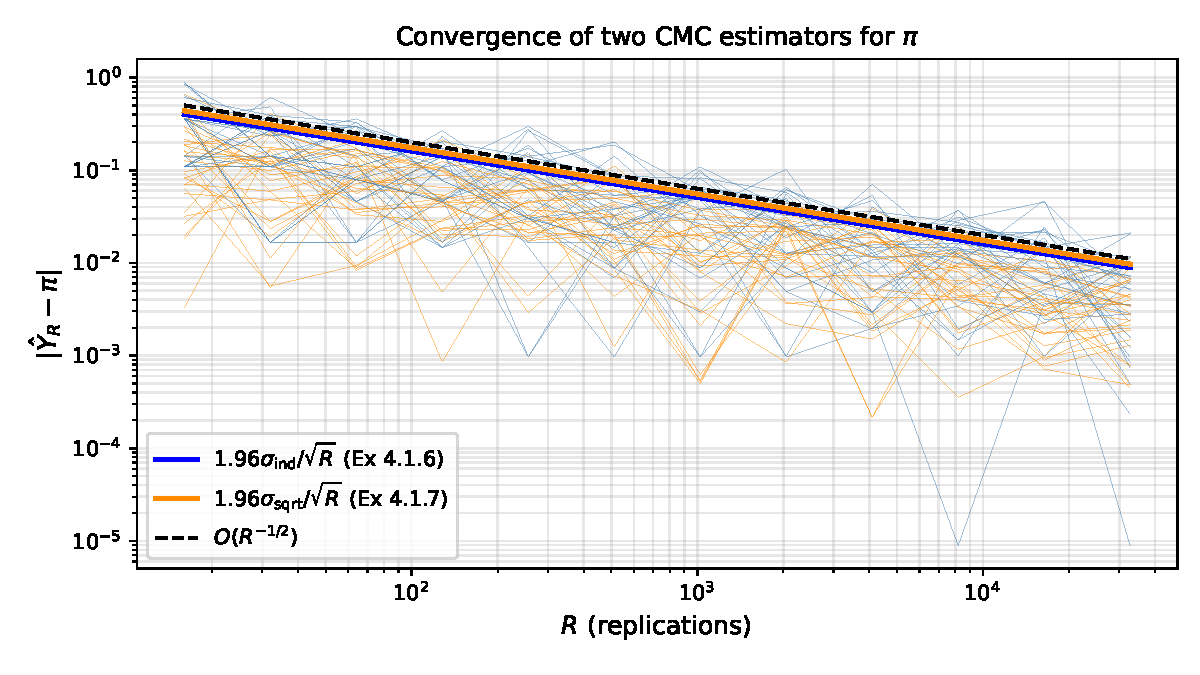
\includegraphics[width=0.72\textwidth]{fig_pi_convergence}
\end{center}

\end{frame}

\begin{frame}[allowframebreaks]{4.1.1 Crude Monte Carlo and Hit-or-Miss Integration}

Computing integrals is a core use case for Monte Carlo.  Suppose we want:
\[
  I = \int_B k(x)\,dx,
\]
where $k : B \to \mathbb{R}$ is an integrable function and $B \subseteq \mathbb{R}^d$
is a bounded set with volume $\mathrm{Vol}(B) = 1$ (rescale if needed; typically
$B = [0,1]^d$).

\begin{block}{Crude Monte Carlo (CMC) Estimator (Eq.\ 1.13)}
  Let $V_1, \ldots, V_R \sim \mathcal{U}(B)$ (uniform on $B$) be i.i.d.
  Setting $Y = k(V)$ ensures $\mathbb{E}Y = \int_B k(v)\,dv = I$.  The CMC
  estimator is:
  \[
    \hat{Y}_R^{\mathrm{CMC}} = \frac{1}{R}\sum_{j=1}^R k(V_j). \tag{1.13}
  \]
  More generally, if $X$ has density $f$ on $B$ and $Y = k(X)$, then
  $\mathbb{E}Y = \int_B k(x) f(x)\,dx = I$, and we average $k(X_j)$ over
  i.i.d.\ draws $X_j \sim f$.
\end{block}

\begin{exampleblock}{Example~4.1.10 (Madras) -- Estimating $I = \int_0^1 k(x)\,dx$}
  Let $k(x) = (e^x - 1)/(e - 1)$.  Setting $Y = k(U)$, $U \sim \mathcal{U}[0,1]$:
  \begin{align*}
    I = \mathbb{E}Y &= \frac{1}{e-1}\!\left(e - 1 - 1\right) = \frac{e-2}{e-1} \approx 0.418. \\
    \mathbb{E}Y^2 &= \int_0^1 k^2(x)\,dx = 0.2567. \\
    \sigma_Y^2 &= 0.2567 - (0.418)^2 = 0.0820.
  \end{align*}
  To achieve precision $b$: $R = 0.3280/b^2$ replications are needed.
\end{exampleblock}

\framebreak

\begin{block}{Hit-or-Miss (HoM) Estimator (Example~4.1.11)}
  Assume $0 \leq k(x) \leq 1$ for all $x \in B = [0,1]$.  Generate
  $U_1, U_2 \sim \mathcal{U}[0,1]$ independently, and define
  $Y' = \mathbf{1}(k(U_1) > U_2)$ (1 if the point $(U_1, U_2)$ lands
  below the curve $k$, 0 otherwise).  Then:
  \[
    \mathbb{E}Y' = \int_0^1 \int_0^{k(u_1)} du_2\,du_1 = \int_0^1 k(u_1)\,du_1 = I.
  \]
  The HoM estimator is $\hat{Y}_R^{\mathrm{HoM}} = \frac{1}{R}\sum_{j=1}^R Y_j'$.
  However, $\mathrm{Var}(Y') = I(1-I) \geq \mathrm{Var}(k(U))$ in general,
  so HoM is \emph{less} statistically efficient than CMC and requires twice
  as many uniform random numbers.  For $k(x) = (e^x-1)/(e-1)$:
  $\mathrm{Var}(Y') \approx 0.2433$, which is about $2.97\times$ the CMC
  variance.  The HoM method is simple but wasteful.
\end{block}

\begin{columns}
  \begin{column}{0.50\textwidth}
    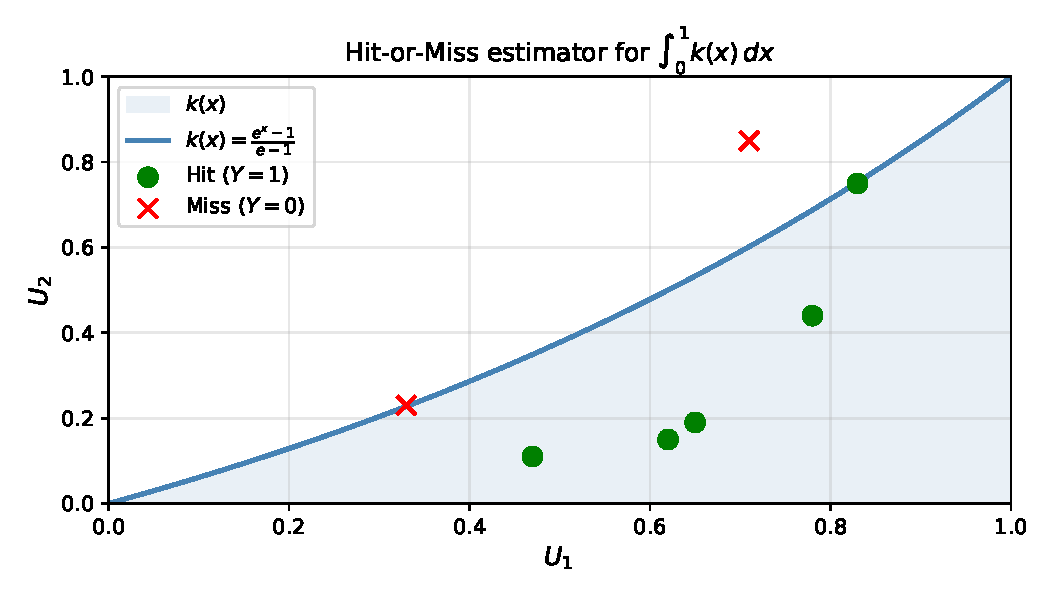
\includegraphics[width=\textwidth]{fig_hit_or_miss}
  \end{column}
  \begin{column}{0.48\textwidth}
    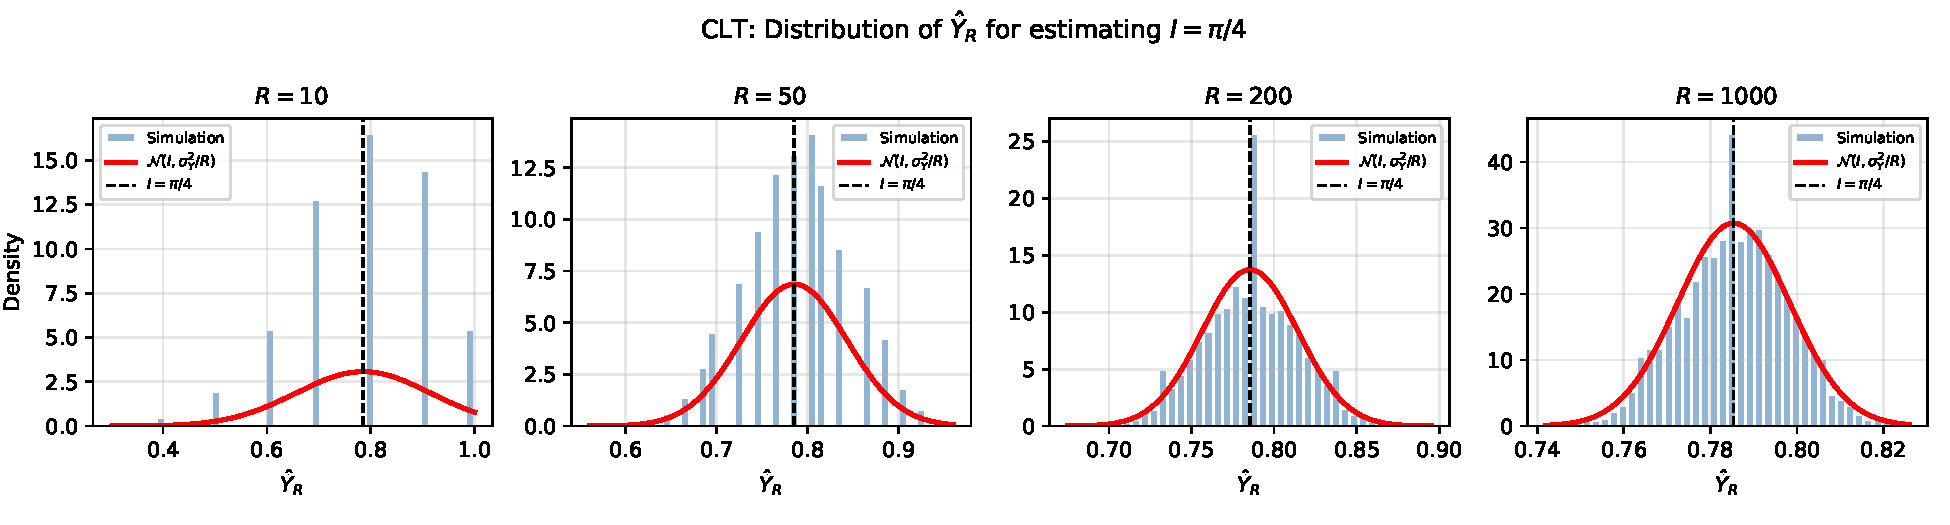
\includegraphics[width=\textwidth]{fig_clt_convergence}
  \end{column}
\end{columns}

\end{frame}

\begin{frame}[allowframebreaks]{4.1.1 Bounding the Variance Without Knowing $I$}

To use formula (1.7) in practice, we need $\sigma_Y^2 = \mathrm{Var}(Y)$.
But $\mathrm{Var}(Y) = \mathbb{E}Y^2 - (\mathbb{E}Y)^2 = \mathbb{E}Y^2 - I^2$,
which involves the unknown $I$.  Sometimes we can bound $\sigma_Y^2$ from above
using only bounds on $k$.

\begin{block}{Variance Bound for CMC (Remark~4.1.12)}
  For $Y = k(X)$ with $X \sim f$ on $B$, we have
  $\sigma_Y^2 = \int_B k^2(x)f(x)\,dx - I^2$.
  If $k(x) \leq k_{\mathrm{up}}$ and $I \geq k_{\mathrm{down}}$ for known
  constants $k_{\mathrm{up}}, k_{\mathrm{down}}$, then:
  \[
    \sigma_Y^2 \leq k_{\mathrm{up}}^2 - k_{\mathrm{down}}^2.
  \]
  Using this upper bound in (1.7) yields a slightly conservative (larger) $R$
  but guarantees the desired confidence level.  In practice, only an upper bound
  on $\sigma_Y^2$ is needed.
\end{block}

\begin{exampleblock}{Bounding Var$(Y)$ for $k(x) = (e^x-1)/(e-1)$ on $[0,1]$}
  Replacing $e \approx 2.71$ conservatively:
  \begin{align*}
    k_{\mathrm{down}} &\geq 0.4157, \quad
    \int_0^1 k^2(x)\,dx \leq k_{\mathrm{up}}^2 \leq 0.2622.
  \end{align*}
  Therefore $\sigma_Y^2 \leq 0.2622 - (0.4157)^2 = 0.0894$, close to the
  exact value $0.0820$ (only 9\% more).  Using this upper bound, the required
  $R$ is only 9\% more than strictly necessary --- a negligible price for
  not needing to know $I$ exactly.
\end{exampleblock}

\begin{center}
  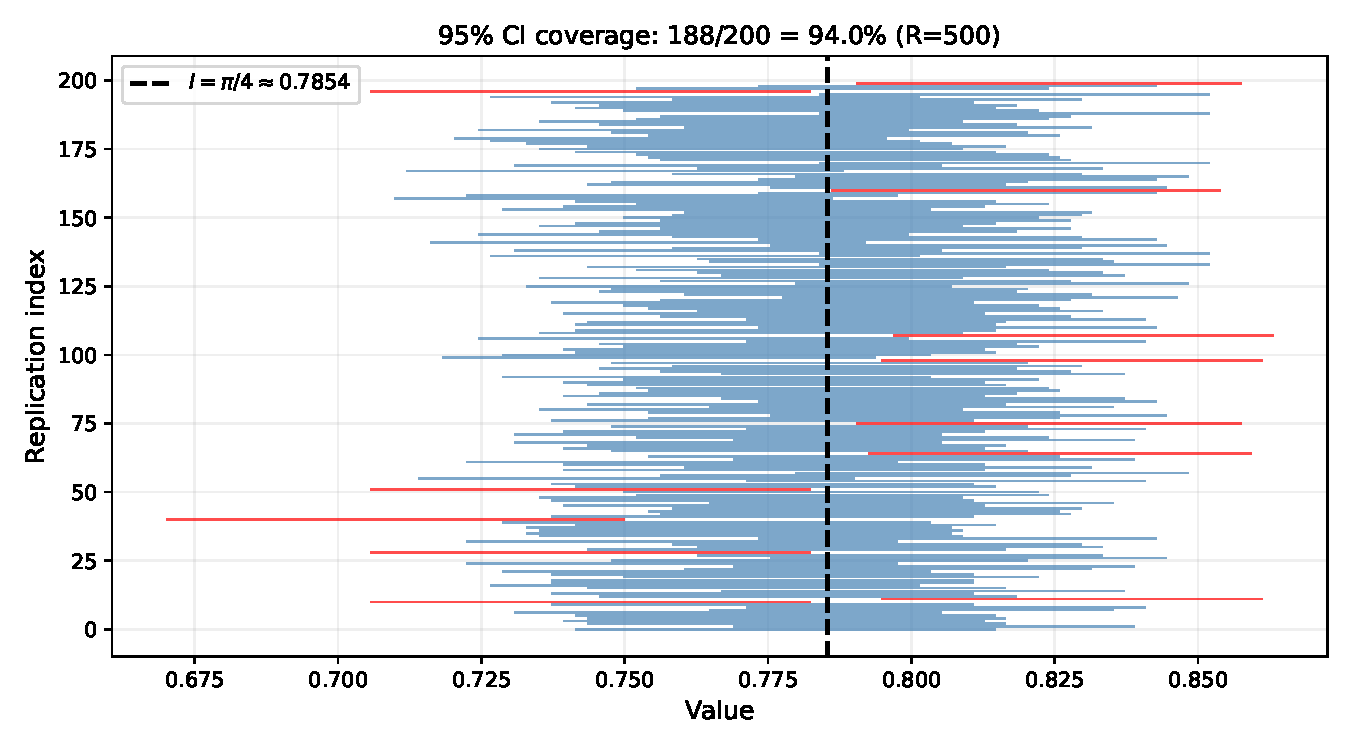
\includegraphics[width=0.60\textwidth]{fig_ci_coverage}
\end{center}

\end{frame}

\begin{frame}[fragile]{4.1.1 Python: Computing a Confidence Interval}
\begin{lstlisting}[style=python]
import numpy as np
from scipy import stats

def estimate_pi_ci(R, alpha=0.05, seed=42):
    """Estimate pi via hit-or-miss MC and report a (1-alpha) CI."""
    rng = np.random.default_rng(seed)
    U = rng.random((R, 2))
    # Y_j = 4 * 1(U1^2 + U2^2 <= 1); E[Y_j] = pi
    Y = 4.0 * (U[:, 0]**2 + U[:, 1]**2 <= 1).astype(float)

    Y_bar = Y.mean()            # sample mean -- estimator of pi
    S2    = Y.var(ddof=1)       # unbiased sample variance (ddof=1 => divide by R-1)
    S     = np.sqrt(S2)

    z      = stats.norm.ppf(1 - alpha / 2)   # z_{1-alpha/2}; for alpha=0.05 => 1.96
    margin = z * S / np.sqrt(R)              # half-width b

    return Y_bar, Y_bar - margin, Y_bar + margin

# Example: R=10000, alpha=0.05
Y_bar, lo, hi = estimate_pi_ci(R=10_000)
print(f"Estimate: {Y_bar:.4f}")
print(f"95% CI : ({lo:.4f}, {hi:.4f})")
print(f"True pi: {np.pi:.4f}")
# Typical output:
# Estimate: 3.1464
# 95% CI : (3.1142, 3.1786)
# True pi: 3.1416
\end{lstlisting}
\end{frame}

%%==================================================================
%% 4.1.2 Multidimensional Case
%%==================================================================

\begin{frame}[allowframebreaks]{4.1.2 The Multidimensional Case}

Sometimes the quantity of interest is a vector
$\mathbf{I} = (I^{(1)}, \ldots, I^{(d)})^T = \mathbb{E}\mathbf{Y}$,
where $\mathbf{Y} = (Y^{(1)}, \ldots, Y^{(d)})^T \in \mathbb{R}^d$.
For instance, we might simultaneously want to estimate the mean height
and mean weight of a population ($d=2$), or compute $d$ different integrals.

\begin{block}{Vector Sample Mean Estimator}
  Given i.i.d.\ replications $\mathbf{Y}_1, \ldots, \mathbf{Y}_R$:
  \[
    \hat{\mathbf{Y}}_R = \frac{1}{R}\sum_{j=1}^R \mathbf{Y}_j
      = \bigl(\hat{Y}_R^{(1)}, \ldots, \hat{Y}_R^{(d)}\bigr)^T,
  \]
  where each component $\hat{Y}_R^{(k)}$ is the sample mean of the $k$-th
  coordinate.  This is unbiased: $\mathbb{E}\hat{\mathbf{Y}}_R = \mathbf{I}$.
\end{block}

Let $\boldsymbol{\Sigma}_{\mathbf{Y}} = \mathbb{E}[(\mathbf{Y}-\mathbf{I})(\mathbf{Y}-\mathbf{I})^T]$
(Sigma bold, a $d\times d$ covariance matrix) capture the variances and
pairwise covariances of the components of $\mathbf{Y}$.  The multivariate CLT:

\begin{block}{Multivariate CLT (Eq.\ 1.23)}
  \[
    \sqrt{R}(\hat{\mathbf{Y}}_R - \mathbf{I}) \;\xrightarrow{\mathcal{D}}\;
      \mathcal{N}\!\left(\mathbf{0},\, \boldsymbol{\Sigma}_{\mathbf{Y}}\right).
  \]
  This means $\hat{\mathbf{Y}}_R$ is approximately
  $\mathcal{N}(\mathbf{I},\, \boldsymbol{\Sigma}_{\mathbf{Y}}/R)$ for large $R$:
  a $d$-dimensional normal distribution centered at the truth, with covariance
  matrix $\boldsymbol{\Sigma}_{\mathbf{Y}}/R$ (shrinking as $1/R$).
\end{block}

\framebreak

\begin{block}{Proposition~4.1.13 -- Key Properties of the Multivariate Normal}
  Let $\mathbf{X} \sim \mathcal{N}(\boldsymbol{\mu}, \boldsymbol{\Sigma})$
  with $\boldsymbol{\Sigma} = \mathbf{A}\mathbf{A}^T$.  Then:
  \begin{enumerate}[(a)]
    \item $\mathbf{Z} = \mathbf{A}^{-1}(\mathbf{X} - \boldsymbol{\mu}) \sim \mathcal{N}(\mathbf{0}, \mathbf{Id}_d)$:
      the standardized vector has independent standard normal components.
    \item $(\mathbf{X}-\boldsymbol{\mu})^T\boldsymbol{\Sigma}^{-1}(\mathbf{X}-\boldsymbol{\mu}) \sim \chi_d^2$
      (chi-squared with $d$ degrees of freedom).
  \end{enumerate}
\end{block}

\textbf{Understanding part (b).}  The expression
$(\mathbf{X}-\boldsymbol{\mu})^T\boldsymbol{\Sigma}^{-1}(\mathbf{X}-\boldsymbol{\mu})$
is the \emph{squared Mahalanobis distance} from $\mathbf{X}$ to $\boldsymbol{\mu}$
(mu, the mean vector) -- it measures how far $\mathbf{X}$ is from its mean in
units of standard deviations, accounting for correlations.  Part (b) says this
distance follows a chi-squared ($\chi^2$, chi-square) distribution with $d$
(d) degrees of freedom.

\textbf{Proof sketch.}  From (a), $\mathbf{Z} \sim \mathcal{N}(\mathbf{0}, \mathbf{Id}_d)$
has i.i.d.\ standard normal components.  Then:
$(\mathbf{X}-\boldsymbol{\mu})^T\boldsymbol{\Sigma}^{-1}(\mathbf{X}-\boldsymbol{\mu})
= \mathbf{Z}^T\mathbf{Z} = \sum_{i=1}^d Z_i^2$,
which is the sum of $d$ squared i.i.d.\ standard normals --- exactly the
definition of $\chi_d^2$.

\textbf{Values of $q_{0.95}(\chi_d^2)$ (the 95th percentile):}
\begin{center}
  \begin{tabular}{cccc}
    \toprule
    $d$ & $q_{0.95}(\chi_d^2)$ & $\sqrt{q}$ (``effective radius'') & Remark \\
    \midrule
    1   & 3.841 & 1.960 & $\pm 1.96\sigma$ interval (familiar 1D result) \\
    2   & 5.991 & 2.448 & confidence ellipse \\
    5   & 11.07 & 3.327 & 5D ellipsoid \\
    10  & 18.31 & 4.279 & 10D ellipsoid \\
    \bottomrule
  \end{tabular}
\end{center}

\end{frame}

\begin{frame}[allowframebreaks]{4.1.2.2 Shapes of Confidence Regions}

For $\mathbf{X} \sim \mathcal{N}(\boldsymbol{\mu}, \boldsymbol{\Sigma})$, a
confidence region $\mathcal{C} \subset \mathbb{R}^d$ satisfying
$\mathbb{P}(\mathbf{X} \in \mathcal{C}) \geq 1-\alpha$ can take three shapes,
each trading off precision against computational cost.

\begin{block}{(1) Confidence Ellipsoid -- Smallest Region (Eq.\ 1.15)}
  Using Proposition 4.1.13(b):
  \[
    \mathcal{C}^{\mathrm{el}} = \bigl\{\mathbf{x} \in \mathbb{R}^d
      : \mathbf{x}^T\boldsymbol{\Sigma}^{-1}\mathbf{x} \leq q_{1-\alpha}(\chi_d^2)\bigr\}
  \]
  satisfies $\mathbb{P}(\mathbf{X} \in \mathcal{C}^{\mathrm{el}}) = 1-\alpha$ exactly.
  This is the \emph{minimum-volume} region achieving coverage $1-\alpha$.
  If $\boldsymbol{\Sigma} = \mathbf{F}\boldsymbol{\Lambda}\mathbf{F}^T$ is the
  eigendecomposition (Lambda = diagonal matrix of eigenvalues $\lambda_i$,
  F = matrix of eigenvectors $\mathbf{f}_i$), the ellipsoid has principal axes
  of half-length $\sqrt{q_{1-\alpha}(\chi_d^2)\,\lambda_i}$ in direction $\mathbf{f}_i$.
\end{block}

\begin{block}{(2) Confidence Parallelogram (Eq.\ 1.18)}
  Since $\boldsymbol{\Sigma}^{-1/2}(\mathbf{X}-\boldsymbol{\mu}) \sim \mathcal{N}(\mathbf{0}, \mathbf{Id}_d)$,
  we choose $z = \Phi^{-1}((\sqrt[d]{1-\alpha}+1)/2)$ and form a hypercube
  $\mathcal{H} = (-z, z)^d$ in the standardized space.  Transforming back:
  \[
    \mathcal{C}^{\mathrm{par}} = \boldsymbol{\Sigma}^{1/2}\mathcal{H} + \boldsymbol{\mu}.
  \]
  This parallelogram has exactly the same coverage $1-\alpha$ as the ellipsoid
  but is generally larger.  Its corners are $\boldsymbol{\Sigma}^{1/2}\mathbf{v} + \boldsymbol{\mu}$
  for $\mathbf{v} = (\pm z, \ldots, \pm z)$.
\end{block}

\begin{block}{(3) Rectangular Confidence Region -- Conservative (Eq.\ 1.19)}
  The axis-aligned rectangle
  $\mathcal{C}^{\mathrm{rec}} = [-c_1, c_1] \times \cdots \times [-c_d, c_d]$
  with $c_i = \sigma_i\,\Phi^{-1}((\sqrt[d]{1-\alpha}+1)/2)$ (where $\sigma_i$
  is the marginal standard deviation of coordinate $i$) satisfies
  $\mathbb{P}(\mathbf{X} \in \mathcal{C}^{\mathrm{rec}}) \geq 1-\alpha$
  (by the \v{S}id\'ak inequality).  This is conservative -- it ignores
  correlations -- but easiest to compute and interpret (it is just
  independent CIs for each component).
\end{block}

\framebreak

\begin{exampleblock}{Example~4.1.14: $\boldsymbol{\Sigma} = \begin{pmatrix}1 & 2 \\ 2 & 6\end{pmatrix}$, $\alpha = 0.05$}
  The covariance matrix has eigenvalues:
  $\lambda_1 = (7+\sqrt{41})/2 \approx 6.7015$,
  $\lambda_2 = (7-\sqrt{41})/2 \approx 0.2984$.
  Eigenvectors: $\mathbf{f}_1 = (-0.3310, -0.9436)^T$, $\mathbf{f}_2 = (-0.9436, 0.3310)^T$.

  At $\alpha = 0.05$: $q_{0.95}(\chi_2^2) = 5.991$.

  \textbf{Ellipsoid} principal axis half-lengths:
  $\sqrt{5.991 \times 6.7015} \approx 6.337$ and $\sqrt{5.991 \times 0.2984} \approx 1.337$.
  The ellipsoid is highly elongated in the $\mathbf{f}_1$ direction.

  \textbf{Parallelogram:} $z = \Phi^{-1}((\sqrt{0.95}+1)/2) = 2.2365$;
  corners $(\pm 2.2365, \pm 2.2365)$ mapped by $\boldsymbol{\Sigma}^{1/2}$.

  \textbf{Rectangle:} $c_1 = 1 \times 2.2365 = 2.2365$, $c_2 = \sqrt{6} \times 2.2365 \approx 5.478$.
  This is conservative: the true rectangular coverage is 95.98\%, slightly above 95\%.
\end{exampleblock}

\begin{center}
  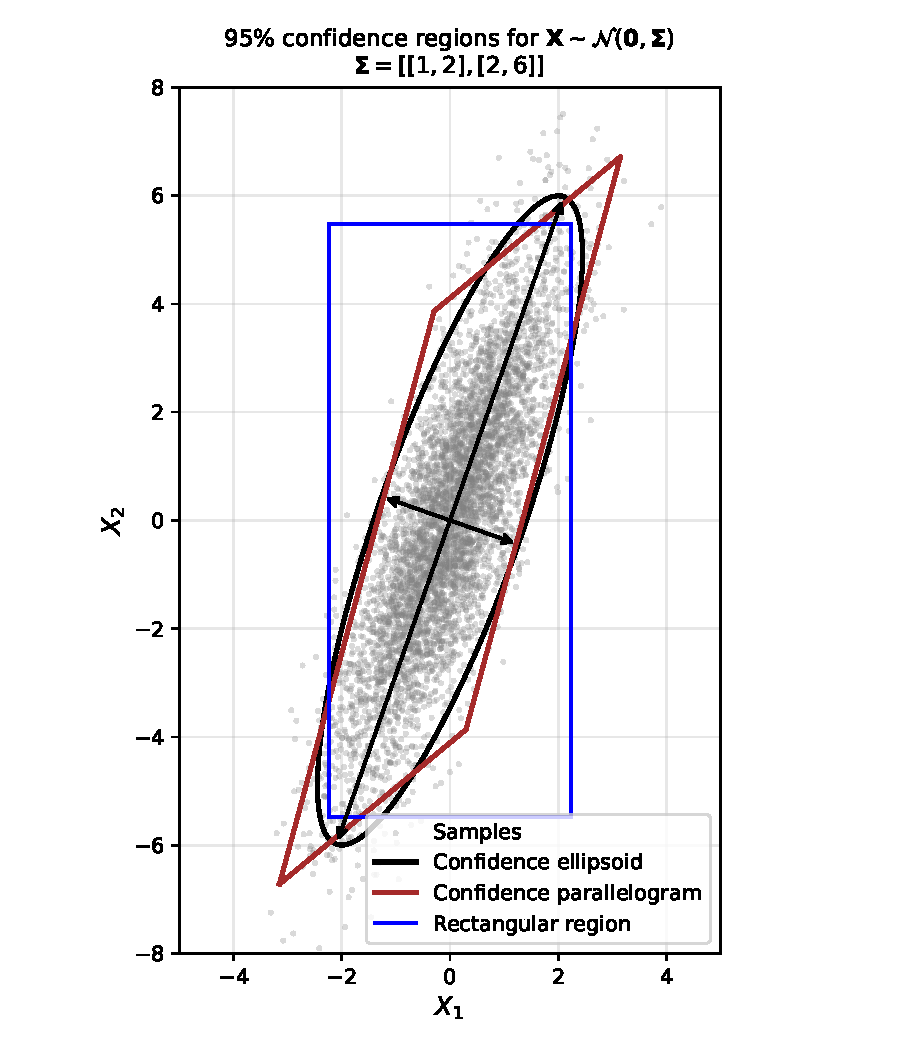
\includegraphics[width=0.42\textwidth]{fig_conf_regions_2d}
\end{center}

\end{frame}

\begin{frame}[allowframebreaks]{4.1.2.3 Confidence Regions for the Estimator $\hat{\mathbf{Y}}_R$}

In practice, we observe the multivariate sample mean $\hat{\mathbf{Y}}_R$,
which by the multivariate CLT is approximately
$\mathcal{N}(\mathbf{I}, \boldsymbol{\Sigma}_{\mathbf{Y}}/R)$.
Replacing $\boldsymbol{\Sigma}$ by $\boldsymbol{\Sigma}_{\mathbf{Y}}/R$,
the confidence ellipsoid becomes centered at $\hat{\mathbf{Y}}_R$ with
principal axes of half-length $\sqrt{q_{1-\alpha}(\chi_d^2)\,\lambda_i/R}$
in direction $\mathbf{f}_i$ (Eq.\ 1.24).

Since $\boldsymbol{\Sigma}_{\mathbf{Y}}$ is unknown, we estimate it by the
\textbf{sample covariance matrix}:

\begin{block}{Sample Covariance Matrix (Eq.\ 1.25)}
  \[
    \hat{\mathbf{S}}_R^2 = \frac{1}{R-1}\sum_{k=1}^R
      (\mathbf{Y}_k - \hat{\mathbf{Y}}_R)(\mathbf{Y}_k - \hat{\mathbf{Y}}_R)^T.
  \]
  This is the unbiased estimator of $\boldsymbol{\Sigma}_{\mathbf{Y}}$.
  The $(i,j)$ entry is $\hat{\mathbf{S}}_R^2(i,j) = \frac{1}{R-1}\sum_{k=1}^R
  (Y_k^{(i)} - \hat{Y}_R^{(i)})(Y_k^{(j)} - \hat{Y}_R^{(j)})$, the
  sample covariance between coordinates $i$ and $j$.
\end{block}

\textbf{Hotelling's $T^2$ (Remark~4.1.15).}  When $\boldsymbol{\Sigma}_{\mathbf{Y}}$
is replaced by $\hat{\mathbf{S}}_R^2$, the statistic
$R(\hat{\mathbf{Y}}_R - \mathbf{I})^T(\hat{\mathbf{S}}_R^2)^{-1}(\hat{\mathbf{Y}}_R - \mathbf{I})$
follows Hotelling's $T^2$-distribution.  For large $R$ this converges to $\chi_d^2$,
justifying the use of chi-square quantiles in practice.

\framebreak

\begin{exampleblock}{Example~4.1.16 -- Heights and Weights ($R=1000$, $d=2$)}
  Using the SOCR HeightsWeights dataset (first 1000 entries).
  Component $Y^{(1)}$: weight (lbs), Component $Y^{(2)}$: height (inches).

  \textbf{Individual 95\% CIs:}
  $\hat{Y}_R^{(1)} = 127.48$, $\hat{S}_R^{(1)} = 11.80$:
  CI for weight: $(126.75,\; 128.21)$.
  $\hat{Y}_R^{(2)} = 68.05$, $\hat{S}_R^{(2)} = 1.94$:
  CI for height: $(67.93,\; 68.17)$.

  \textbf{Sample covariance and eigendecomposition:}
  \[
    \hat{\mathbf{S}}_R^2 = \begin{pmatrix} 139.29 & 11.40 \\ 11.40 & 3.75 \end{pmatrix},
    \quad \lambda_1 = 140.24,\;\lambda_2 = 2.79.
  \]
  $\mathbf{f}_1 \approx (0.9965, 0.0832)^T$ (mostly along the weight axis),
  $\mathbf{f}_2 \approx (-0.0832, 0.9965)^T$.
  With $q_{0.95}(\chi_2^2) = 5.991$:
  axis half-lengths $\sqrt{5.991 \times 140.24/1000} \approx 0.916$
  and $\sqrt{5.991 \times 2.79/1000} \approx 0.129$.
  The confidence ellipse is extremely elongated along the weight direction,
  reflecting that weight varies much more than height across individuals.
\end{exampleblock}

\end{frame}

\begin{frame}[fragile]{4.1.2 Python: Multivariate Confidence Ellipsoid}
\begin{lstlisting}[style=python]
import numpy as np
from scipy.stats import chi2

def conf_ellipsoid(Y_samples, alpha=0.05):
    """Confidence ellipsoid for the mean of d-dimensional i.i.d. samples."""
    R, d = Y_samples.shape
    Y_bar = Y_samples.mean(axis=0)          # sample mean (d-vector)

    diff = Y_samples - Y_bar
    S2   = (diff.T @ diff) / (R - 1)        # sample covariance matrix (d x d)
    eigvals, eigvecs = np.linalg.eigh(S2)   # eigendecomposition
    q = chi2.ppf(1 - alpha, df=d)           # chi-square quantile at level 1-alpha

    # Half-lengths of principal axes of the confidence ellipsoid
    # Each axis: sqrt(q * lambda_i / R) in direction eigvec[:,i]
    axis_lengths = np.sqrt(q * eigvals / R)
    return Y_bar, axis_lengths, eigvecs, S2

# Simulate 2D example: I = (2.0, 3.0), Sigma = [[1, 0.5],[0.5, 2]]
rng   = np.random.default_rng(42)
Sigma = np.array([[1., 0.5], [0.5, 2.]])
L     = np.linalg.cholesky(Sigma)           # Cholesky factor of Sigma
R     = 1000
Y     = (L @ rng.standard_normal((2, R))).T + np.array([2.0, 3.0])

Y_bar, axes, vecs, S2 = conf_ellipsoid(Y, alpha=0.05)
print(f"Estimated mean       : {Y_bar}")
print(f"True mean            : [2.0, 3.0]")
print(f"Ellipsoid axis lengths: {axes}")
\end{lstlisting}
\end{frame}

%%==================================================================
%% SECTION 4.2 ESTIMATION OF k(I)
%%==================================================================

\begin{frame}[allowframebreaks]{4.2 Estimation of $k(I)$: Motivation}

In many applications, the quantity of interest is not $I = \mathbb{E}Y$ itself,
but a smooth transformation $z = k(I)$ of the mean.  Examples:

\begin{itemize}
  \item \textbf{Life insurance net premium:}
    $\Pi = r\,\mathbb{E}e^{-rT}/(1-\mathbb{E}e^{-rT}) = k(I)$,
    where $I = \mathbb{E}e^{-rT}$ and $T$ is the insured's future lifetime,
    $r$ is the interest rate.
  \item \textbf{Standard deviation:} $k(I) = \sqrt{I}$ where $I = \mathbb{E}Y^2 - (\mathbb{E}Y)^2$.
  \item \textbf{Ratio of expectations:} $z = I^{(1)}/I^{(2)}$, e.g.\ expected cost
    per unit of expected throughput.
\end{itemize}

\begin{block}{Problem Setup and Natural Estimator}
  Let $k : \mathbb{R}^d \to \mathbb{R}$ be a prescribed continuous function,
  $\mathbf{I} = \mathbb{E}\mathbf{Y}$, and $\hat{\mathbf{X}}_R$ be a
  strongly consistent estimator of $\mathbf{I}$.  The natural estimator of
  $z = k(\mathbf{I})$ is $\hat{Z}_R = k(\hat{\mathbf{X}}_R)$.
  The \textbf{asymptotic variance} (also called the Time Average Variance
  Constant, TAVC) is:
  \[
    \varsigma^2 = \lim_{R\to\infty} R\,\mathrm{Var}(\hat{Z}_R).
  \]
  Here $\varsigma$ (varsigma) is the asymptotic standard deviation constant.
\end{block}

\textbf{Important caveat: $k(\hat{X}_R)$ is generally biased.}
Even when $\hat{X}_R$ is unbiased for $I$, $k(\hat{X}_R)$ is generally biased
for $k(I)$ because of the nonlinearity of $k$.  For example, with $k(y) = y^2$:
$\mathbb{E}[\hat{Y}_R^2] = (\mathbb{E}Y)^2 + R^{-1}\sigma_Y^2 \neq (\mathbb{E}Y)^2$.
However, the bias is $O(R^{-1})$ while the standard deviation is $O(R^{-1/2})$,
so for large $R$ the bias is negligible relative to the uncertainty.

\end{frame}

\begin{frame}[allowframebreaks]{4.2.1 The Delta Method (Case $\hat{X}_R = \hat{Y}_R$)}

The key tool is the \textbf{delta method}.  The idea: if $k$ is smooth and
$\hat{Y}_R \approx I$ for large $R$, we linearize $k(\hat{Y}_R)$ around $I$
using a Taylor expansion.

\begin{block}{Taylor Expansion Argument}
  If $k$ is continuously differentiable near $I$:
  \[
    k(x) - k(I) = k'(I)(x - I) + o(x - I) \quad \text{as } x \to I.
  \]
  Substituting $x = \hat{Y}_R$ and multiplying by $\sqrt{R}$:
  \[
    \sqrt{R}\bigl(k(\hat{Y}_R) - k(I)\bigr) = k'(I)\cdot\underbrace{\sqrt{R}(\hat{Y}_R - I)}_{\xrightarrow{\mathcal{D}}\,\mathcal{N}(0,\sigma_Y^2)}
      + \underbrace{\sqrt{R}\cdot o(\hat{Y}_R - I)}_{\to\,0\;\text{in prob.}}
  \]
  The remainder vanishes because $\sqrt{R}|\hat{Y}_R - I|$ is bounded in
  probability (by the CLT) while $o(|\hat{Y}_R-I|)/|\hat{Y}_R-I| \to 0$.
\end{block}

\begin{block}{Proposition~4.2.1 -- Delta Method, 1D Version (Eq.\ 2.2)}
  Let $Y_1, Y_2, \ldots$ be i.i.d., $\hat{Y}_R = \frac{1}{R}\sum Y_j$,
  $I = \mathbb{E}Y$, $\sigma_Y^2 = \mathrm{Var}(Y)$, and $k$ continuously
  differentiable at $I$.  Then:
  \[
    \sqrt{R}\bigl(k(\hat{Y}_R) - k(I)\bigr) \;\xrightarrow{\mathcal{D}}\; \mathcal{N}(0, \varsigma^2),
    \quad \varsigma^2 = k'(I)^2\,\sigma_Y^2.
  \]
  Here $k'(I)$ (k prime of I) is the derivative of $k$ evaluated at the true
  value $I$, and $\sigma_Y^2$ is the variance of a single observation.
  The asymptotic variance $\varsigma^2$ is the product of the squared
  derivative (which amplifies or shrinks the uncertainty) and the single-sample
  variance.
\end{block}

\framebreak

Since $I$ and $\sigma_Y^2$ are unknown, we replace them by $\hat{Y}_R$
and $\hat{S}_R^2$ (both are consistent), giving the practical CI:

\begin{block}{Practical CI for $k(I)$ at Level $1-\alpha$ (Eq.\ 2.3)}
  \[
    \left(k(\hat{Y}_R) - z_{1-\alpha/2}\,\frac{\hat{S}_R\,|k'(\hat{Y}_R)|}{\sqrt{R}},\;\;
    k(\hat{Y}_R) + z_{1-\alpha/2}\,\frac{\hat{S}_R\,|k'(\hat{Y}_R)|}{\sqrt{R}}\right). \tag{2.3}
  \]
  The half-width is $z_{1-\alpha/2}\,\hat{S}_R\,|k'(\hat{Y}_R)|/\sqrt{R}$.
  This CI is asymptotically valid.  The factor $|k'(\hat{Y}_R)|$ stretches
  or shrinks the uncertainty: where $k$ is steep, the CI is wide; where
  $k$ is flat, the CI is narrow.
\end{block}

\begin{exampleblock}{Example~4.2.2 -- Life Insurance Net Premium}
  The net premium for whole-life assurance at interest rate $r$ (r) is
  $\Pi = r\,\mathbb{E}e^{-rT}/(1 - \mathbb{E}e^{-rT}) = k(I)$,
  where $I = \mathbb{E}e^{-rT}$ and $T = T_x$ is the future lifetime.
  Set $Y = e^{-rT}$ so $\hat{Y}_R = \frac{1}{R}\sum e^{-rT_j}$ estimates $I$.
  The function $k(x) = rx/(1-x)$ has derivative $k'(x) = r/(1-x)^2$.
  The CI (2.3) becomes:
  \[
    k(\hat{Y}_R) \;\pm\; \frac{z_{1-\alpha/2}\,r\,\hat{S}_R}{(1-\hat{Y}_R)^2\sqrt{R}}.
  \]
  Notice: as $\hat{Y}_R \to 1$ (corresponding to very long expected lifetime
  or high interest rate), the factor $(1-\hat{Y}_R)^2$ in the denominator
  becomes tiny, causing the CI to widen dramatically --- the premium becomes
  very sensitive to estimation error in $I$.
\end{exampleblock}

\begin{center}
  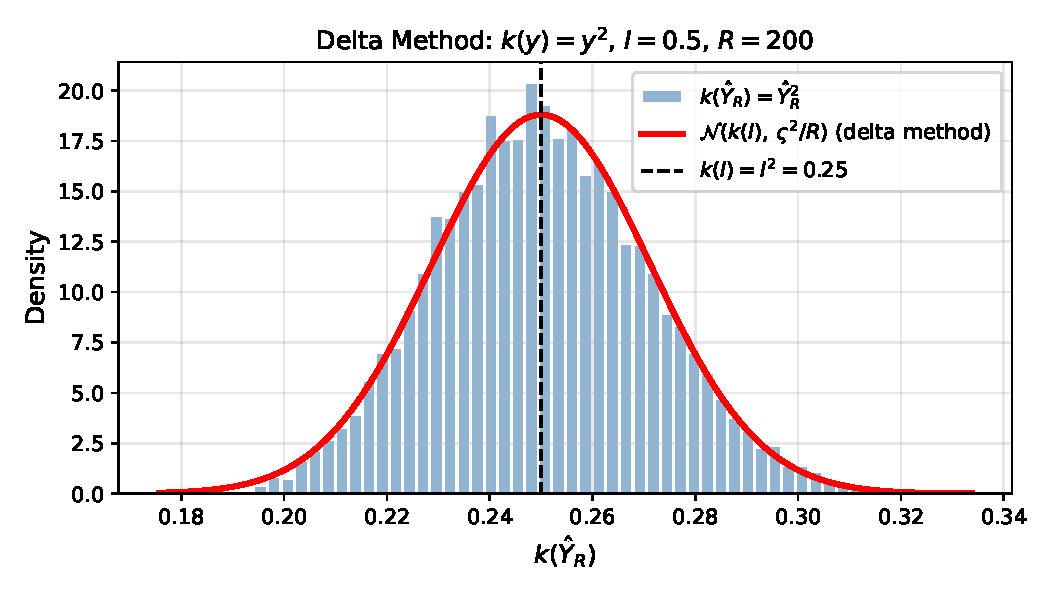
\includegraphics[width=0.48\textwidth]{fig_delta_method}
\end{center}

\end{frame}

\begin{frame}[allowframebreaks]{4.2.1 Multidimensional Delta Method}

When $\mathbf{I} = \mathbb{E}\mathbf{Y}$ is $d$-dimensional and
$k : \mathbb{R}^d \to \mathbb{R}$, the delta method generalizes using the
gradient $\nabla k$ (nabla k, meaning the vector of partial derivatives).

\begin{block}{Two-Dimensional Case (Proposition~4.2.3, Eq.\ 2.5--2.6)}
  Let $\mathbf{Y}_j = (Y_j^{(1)}, Y_j^{(2)})^T$ be i.i.d.,
  $\mathbf{I} = (I^{(1)}, I^{(2)})^T$, and $k(y_1, y_2)$ continuously
  differentiable at $\mathbf{I}$.  Then:
  \[
    \sqrt{R}(k(\hat{\mathbf{Y}}_R) - k(\mathbf{I})) \;\xrightarrow{\mathcal{D}}\;
      \mathcal{N}(0, \varsigma^2),
  \]
  where the asymptotic variance uses the covariance matrix
  $\boldsymbol{\Sigma}_{\mathbf{Y}}$ (entries: $\boldsymbol{\Sigma}_{\mathbf{Y}}(i,j)
  = \mathrm{Cov}(Y^{(i)}, Y^{(j)})$):
  \[
    \varsigma^2 = (k'_{y_1})^2\boldsymbol{\Sigma}_{\mathbf{Y}}(1,1)
      + (k'_{y_2})^2\boldsymbol{\Sigma}_{\mathbf{Y}}(2,2)
      + 2k'_{y_1}k'_{y_2}\boldsymbol{\Sigma}_{\mathbf{Y}}(1,2), \tag{2.6}
  \]
  with $k'_{y_i} = \partial k/\partial y_i|_{\mathbf{y}=\mathbf{I}}$
  (partial derivative of $k$ with respect to $y_i$, evaluated at $\mathbf{I}$).
\end{block}

\begin{block}{General $d$-Dimensional Case (Proposition~4.2.8, Eq.\ 2.15)}
  If $k : \mathbb{R}^d \to \mathbb{R}$ is continuously differentiable at $\mathbf{I}$:
  \[
    \varsigma^2 = \nabla k(\mathbf{I})\,\boldsymbol{\Sigma}_{\mathbf{Y}}\,(\nabla k(\mathbf{I}))^T
      = \sum_{i,j=1}^d k^{(i)}(\mathbf{I})\,k^{(j)}(\mathbf{I})\,\boldsymbol{\Sigma}_{\mathbf{Y}}(i,j), \tag{2.15}
  \]
  where $k^{(i)}(\mathbf{I}) = \partial k/\partial x_i|_{\mathbf{x}=\mathbf{I}}$.
  This is a quadratic form (a weighted sum of products) in the gradient of $k$.
\end{block}

\framebreak

In practice, we estimate the unknown $\mathbf{I}$ and $\boldsymbol{\Sigma}_{\mathbf{Y}}$
by $\hat{\mathbf{Y}}_R$ and $\hat{\mathbf{S}}_R^2$.  The estimated asymptotic
variance is (Eq.\ 2.16):
\[
  \hat{\varsigma}^2 = \sum_{i,j=1}^d k^{(i)}(\hat{\mathbf{Y}}_R)\,k^{(j)}(\hat{\mathbf{Y}}_R)\,
    \hat{\mathbf{S}}_R^2(i,j).
\]
The practical CI at level $1-\alpha$ is:
\[
  k(\hat{\mathbf{Y}}_R) \;\pm\; z_{1-\alpha/2}\,\frac{\hat{\varsigma}}{\sqrt{R}}.
  \quad \text{(Eq.\ 2.8)}
\]

\begin{exampleblock}{Example~4.2.5 -- Ratio of Expectations $z = I^{(1)}/I^{(2)}$}
  Estimate the ratio $z = I^{(1)}/I^{(2)}$ using
  $\hat{Z}_R = \hat{Y}_R^{(1)}/\hat{Y}_R^{(2)}$.
  With $k(y_1, y_2) = y_1/y_2$: partial derivatives
  $k'_{y_1} = 1/y_2$ and $k'_{y_2} = -y_1/y_2^2$.
  The asymptotic variance simplifies to:
  \[
    \varsigma^2 = \frac{\mathbb{E}(Y^{(1)} - z Y^{(2)})^2}{(I^{(2)})^2},
  \]
  estimated from data as (Eq.\ 2.13):
  \[
    \widehat{\mathrm{Var}}(\hat{Z}_R) = \frac{1}{R^2(\hat{Y}_R^{(2)})^2}
      \sum_{i=1}^R (Y_i^{(1)} - \hat{Z}_R\,Y_i^{(2)})^2.
  \]
  The CI is: $\hat{Z}_R \pm z_{1-\alpha/2}\sqrt{\widehat{\mathrm{Var}}(\hat{Z}_R)}$.
\end{exampleblock}

\end{frame}

\begin{frame}[allowframebreaks]{4.2.2 General Consistent Estimator $\hat{X}_R$ and Asymptotic Bias}

The delta method extends to any strongly consistent estimator $\hat{X}_R \to I$
satisfying:
\begin{enumerate}[(A1)]
  \item $\sqrt{R}(\hat{X}_R - \mathbb{E}\hat{X}_R) \xrightarrow{\mathcal{D}} \mathcal{N}(0, \sigma^2)$
    (asymptotically normal when centered at its own mean).
  \item $\sqrt{R}(\mathbb{E}\hat{X}_R - I) \to 0$ as $R \to \infty$
    (the bias vanishes faster than $1/\sqrt{R}$).
\end{enumerate}
Under (A1) and (A2): $\sqrt{R}(\hat{X}_R - I) \xrightarrow{\mathcal{D}} \mathcal{N}(0, \sigma^2)$.
For $\hat{Z}_R = k(\hat{X}_R)$, the same delta method gives
$\varsigma^2 = k'(I)^2\,\sigma^2$.

\begin{block}{Asymptotic Bias of $\hat{Z}_R$ (Eq.\ 2.17)}
  Under assumption (A2$'$): $R(\mathbb{E}\hat{X}_R - I) \to \beta^X$
  (the bias of $\hat{X}_R$ is of order $R^{-1}$ with constant $\beta^X$),
  the $R^{-1}$-order asymptotic bias of $\hat{Z}_R = k(\hat{X}_R)$ is:
  \[
    \beta^Z = \beta^X k'(I) + \frac{\sigma^2 k''(I)}{2}. \tag{2.17}
  \]
  Here $k''(I)$ (k double-prime of I) is the second derivative of $k$ at $I$.
  The first term $\beta^X k'(I)$ propagates the bias of $\hat{X}_R$ through $k$.
  The second term $\sigma^2 k''(I)/2$ is the \emph{Jensen's inequality effect}:
  the curvature of $k$ creates bias even when $\hat{X}_R$ is perfectly unbiased
  ($\beta^X = 0$).  A bias-corrected estimator is $k(\hat{X}_R) - \hat{\beta}^Z/R$,
  but this correction is usually negligible because std dev $O(R^{-1/2})$
  dominates bias $O(R^{-1})$ for large $R$ (Remark~4.2.4).
\end{block}

\framebreak

\begin{block}{4.2.3 Mean Square Error, Bias, and Variance (Eq.\ 2.19)}
  For any estimator $\hat{X}_R$ of $I$:
  \[
    \mathrm{MSE}(\hat{X}_R) = \mathbb{E}(\hat{X}_R - I)^2
      = \underbrace{\mathrm{Var}(\hat{X}_R)}_{\text{variance}} + \underbrace{(\mathbb{E}\hat{X}_R - I)^2}_{\text{squared bias}}.
  \]
  Variance measures random fluctuation; squared bias measures systematic
  error.  An unbiased estimator has MSE = Variance.
\end{block}

For large $R$, using $\lim_{R\to\infty} R\,\mathrm{Var}(\hat{X}_R) = \varsigma^2$
and $\lim_{R\to\infty} R(\mathbb{E}\hat{X}_R - I) = \beta$:
\[
  \mathrm{MSE}(\hat{X}_R) \approx \frac{\varsigma^2}{R} + \frac{\beta^2}{R^2}.
\]
The variance term is $O(R^{-1})$ and the squared bias is $O(R^{-2})$ ---
the bias is negligible for large $R$, justifying ignoring bias corrections.

\begin{exampleblock}{Example~4.2.9 -- $k(y) = y^2$}
  Let $\hat{Z}_R = \hat{Y}_R^2$.  Then $k'(y) = 2y$, $k''(y) = 2$.
  Since $\hat{Y}_R$ is unbiased ($\beta^X = 0$), formula (2.17) gives:
  $\beta^Z = 0 + \sigma_Y^2 \cdot 2/2 = \sigma_Y^2$.
  We can verify directly: $\mathbb{E}(\hat{Y}_R)^2 = (\mathbb{E}Y)^2 + \mathrm{Var}(\hat{Y}_R)
  = k(I) + \sigma_Y^2/R$.
  So $\hat{Y}_R^2$ overestimates $I^2$ by $\sigma_Y^2/R$ on average.
  The delta method asymptotic variance: $\varsigma^2 = (2I)^2\sigma_Y^2 = 4I^2\sigma_Y^2$.
\end{exampleblock}

\begin{center}
  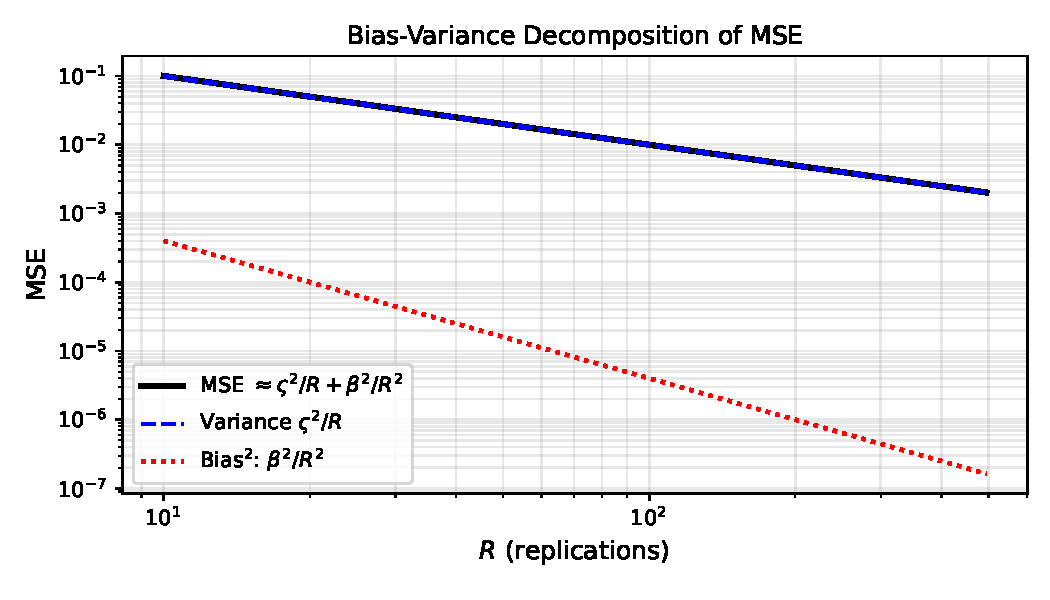
\includegraphics[width=0.55\textwidth]{fig_mse_decomp}
\end{center}

\end{frame}

\begin{frame}[fragile]{4.2 Python: Delta Method Confidence Interval}
\begin{lstlisting}[style=python]
import numpy as np
from scipy import stats

def delta_method_ci(Y_samples, k_func, k_prime, alpha=0.05):
    """
    Compute CI for k(I) using the delta method.
    Y_samples : 1D array of i.i.d. realizations of Y (E[Y]=I)
    k_func    : callable, the transformation k
    k_prime   : callable, derivative k' (evaluated at a scalar)
    """
    R     = len(Y_samples)
    Y_bar = Y_samples.mean()
    S     = Y_samples.std(ddof=1)    # sample std dev

    z_est    = k_func(Y_bar)                          # point estimate
    asymp_std = abs(k_prime(Y_bar)) * S / np.sqrt(R) # estimated asymptotic std dev

    z_q = stats.norm.ppf(1 - alpha / 2)
    return z_est, z_est - z_q * asymp_std, z_est + z_q * asymp_std

# Example: k(y) = y^2. Y ~ N(0.5, 0.3^2), I=0.5, k(I)=0.25.
rng = np.random.default_rng(42)
Y   = rng.normal(0.5, 0.3, size=1000)
est, lo, hi = delta_method_ci(
    Y, k_func=lambda y: y**2, k_prime=lambda y: 2*y)
print(f"k(I) estimate: {est:.4f}")
print(f"95% CI:        ({lo:.4f}, {hi:.4f})")
print(f"True k(I)=0.25. Bias: {est - 0.25:.4f}  (expect ~sigma^2/R=0.09/1000=9e-5)")
# Typical output:
# k(I) estimate: 0.2594
# 95% CI:        (0.2399, 0.2789)
\end{lstlisting}
\end{frame}

%%==================================================================
%% SECTION 4.3 QUANTILE ESTIMATION
%%==================================================================

\begin{frame}[allowframebreaks]{4.3 Estimators of a Quantile: Setup and Motivation}

So far we have estimated \emph{means} $I = \mathbb{E}X$.  A quantile is a
completely different summary of a distribution.  The $p$-th quantile is the
value below which a fraction $p$ (p, a number between 0 and 1) of the
probability lies.  In financial risk management, quantiles are called
\textbf{Value-at-Risk (VaR)}: the 99th percentile of losses is the amount
that will only be exceeded 1\% of the time.

\begin{block}{Definition: $p$-th Quantile}
  Let $X \sim F$ (with continuous distribution function $F$ and density $f$).
  The $p$-th quantile for $p \in (0,1)$ is the generalized inverse:
  \[
    q_p = F^{\leftarrow}(p) = \inf\{x : F(x) \geq p\}.
  \]
  For a continuous $F$, this is the unique solution to $F(q_p) = p$.
  In other words, $q_p$ is the value such that exactly a fraction $p$ of
  the distribution lies below it.  The 50th percentile ($p=0.5$) is the median.
\end{block}

Given an i.i.d.\ sample $X_1, \ldots, X_R$ from $F$, the natural estimator
is the \textbf{sample quantile}.  Sort the observations to get
$X_{(1)} \leq X_{(2)} \leq \cdots \leq X_{(R)}$ (order statistics).
The empirical quantile function is (Eq.\ 3.1):
\[
  \hat{F}_R^{\leftarrow}(p) = \begin{cases}
    X_{(\lfloor pR\rfloor)} & \text{if } pR \in \mathbb{Z}, \\
    X_{(\lfloor pR\rfloor+1)} & \text{otherwise.}
  \end{cases}
\]
Here $\lfloor pR \rfloor$ (floor of $pR$) is the largest integer not exceeding $pR$.
For asymptotic analysis we use the simplified estimator $\hat{q}_p = X_{(\lfloor pR\rfloor)}$.

\framebreak

\begin{block}{Proposition~4.3.1 -- Asymptotic Normality of Sample Quantile (Eq.\ 3.2)}
  Assume $f$ is continuous and positive near $q_p$.  Then:
  \begin{enumerate}[(i)]
    \item $\hat{q}_p = X_{(\lfloor pR\rfloor)}$ is a strongly consistent
      estimator of $q_p$.
    \item $\sqrt{R}(\hat{q}_p - q_p) \xrightarrow{\mathcal{D}} \mathcal{N}(0, \varsigma^2)$,
      where
      \[
        \varsigma^2 = \frac{p(1-p)}{f(q_p)^2}.
      \]
  \end{enumerate}
  Here $p$ is the quantile level, $1-p$ is the complementary probability,
  and $f(q_p)$ (f evaluated at $q_p$) is the density of $X$ at the quantile.
\end{block}

\begin{alertblock}{How to Read the Asymptotic Variance $\varsigma^2 = p(1-p)/f(q_p)^2$}
  The variance is \emph{large} when $f(q_p)$ is small (the density is low at
  the quantile, meaning the distribution is spread out there, making the
  quantile hard to pin down precisely) and \emph{small} when $f(q_p)$ is
  large (the distribution has a sharp peak near $q_p$, making the quantile
  easy to locate).  The numerator $p(1-p)$ is maximized at $p=0.5$ (median)
  and decreases toward the tails --- but this is typically dominated by the
  denominator $f(q_p)^2$.
\end{alertblock}

\framebreak

\textbf{Proof sketch (two key steps):}

\textbf{Step 1.}  The $\lfloor Rp\rfloor$-th order statistic of $R$ i.i.d.\
$\mathcal{U}[0,1]$ variables has a $\mathrm{Beta}(\lfloor Rp\rfloor, R - \lfloor Rp\rfloor)$
distribution (Lemma~4.3.2).  Using the representation as ratios of Erlang
variables and the CLT:
\[
  \sqrt{R}(U_{\lfloor Rp\rfloor} - p) \;\xrightarrow{\mathcal{D}}\; \mathcal{N}(0, p(1-p)).
\]

\textbf{Step 2.}  Since $X_{(\lfloor Rp\rfloor)} = F^{\leftarrow}(U_{\lfloor Rp\rfloor})$,
apply the quantile function's Taylor expansion:
$F^{\leftarrow}(p + x) \approx F^{\leftarrow}(p) + x/f(q_p)$.
This rescales the variance by $(1/f(q_p))^2$, giving $\varsigma^2 = p(1-p)/f(q_p)^2$.

\begin{exampleblock}{Worked Example: $X \sim \mathrm{Exp}(1)$, $p = 0.9$}
  The exponential distribution has $F(x) = 1 - e^{-x}$ and $f(x) = e^{-x}$.
  \[
    q_{0.9} = -\ln(0.1) = \ln(10) \approx 2.303.
  \]
  The density at the quantile: $f(q_{0.9}) = e^{-\ln 10} = 1/10 = 0.1$.
  \[
    \varsigma^2 = \frac{0.9 \times 0.1}{0.1^2} = \frac{0.09}{0.01} = 9.
  \]
  For $R = 1{,}000$: standard error $\approx 3/\sqrt{1000} \approx 0.095$.
  The 95\% CI half-width: $1.96 \times 0.095 \approx 0.186$.
  CI: approximately $(2.117,\; 2.489)$.  The large variance ($\varsigma^2 = 9$)
  makes sense: the exponential distribution's density at its 90th percentile
  ($f = 0.1$) is small, meaning it is quite spread out there.
\end{exampleblock}

\begin{center}
  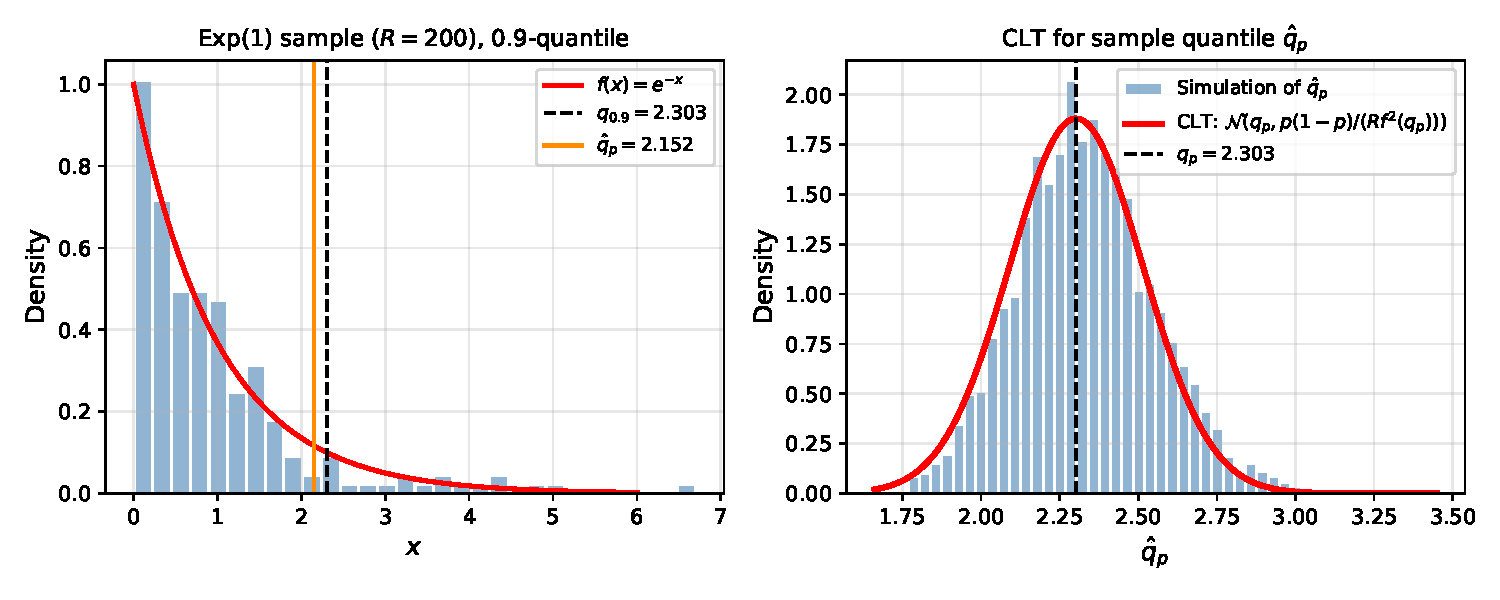
\includegraphics[width=0.60\textwidth]{fig_quantile_estimation}
\end{center}

\end{frame}

\begin{frame}[allowframebreaks]{4.3.1 Estimating $1/f(q_p)$ via Order Statistics}

The confidence interval for $q_p$ requires knowing $\varsigma^2 = p(1-p)/f(q_p)^2$,
hence we need to estimate $1/f(q_p)$.  The quantile function $Q(p) = F^{-1}(p)$
satisfies $Q'(p) = 1/f(Q(p))$, so we want to estimate the derivative $Q'(p)$
at the point $p$.  A natural approach is the finite-difference approximation:
\[
  Q'(p) \approx \frac{Q(p + m/R) - Q(p - m/R)}{2m/R},
\]
for a small bandwidth $m$ (m).  Replacing $Q(p \pm m/R)$ by the corresponding
order statistics gives:

\begin{block}{Order-Statistic Estimator of $Q'(p) = 1/f(q_p)$ (Proposition~4.3.4, Eq.\ 3.3)}
  Choose bandwidth $m = m_R$ (a positive integer) and define:
  \[
    \hat{Q}'_{p,R} = \frac{R}{2m}\Bigl(X_{(\lfloor pR\rfloor + m)}
      - X_{(\lfloor pR\rfloor - m + 1)}\Bigr). \tag{3.3}
  \]
  Intuition: $X_{(\lfloor pR\rfloor + m)}$ estimates $Q(p + m/R)$ and
  $X_{(\lfloor pR\rfloor - m + 1)}$ estimates $Q(p - m/R)$; dividing the
  difference by $2m/R$ approximates $Q'(p)$.

  \textbf{Consistency:} If $f$ has a continuous derivative near $q_p$ and
  $m_R \to \infty$ with $m_R = o(R)$ (grows but slower than $R$), then
  $\hat{Q}'_{p,R} \to Q'(p) = 1/f(q_p)$ with probability~1.
\end{block}

\textbf{Choosing the bandwidth $m_R$:}

\begin{itemize}
  \item \textbf{Simple rule:} $m_R = \lfloor\sqrt{R}\rfloor$ (floor of square root of R).
    Satisfies both $m_R \to \infty$ and $m_R = o(R)$.  Default choice in practice.
    For $R = 10{,}000$: $m_R = 100$.
  \item \textbf{MSE-optimal (Bloch--Gastwirth):} $m_R = cR^{4/5}$ minimizes the
    asymptotic MSE of $\hat{Q}'_{p,R}$, with MSE $\sim C \cdot R^{-2/5}$ (slower
    than $R^{-1/2}$, reflecting the fundamental difficulty of density estimation).
\end{itemize}

\begin{block}{Confidence Interval for $q_p$ (combining Prop.\ 4.3.1 and 4.3.4)}
  Substituting $\hat{Q}'_{p,R}$ for $1/f(q_p)$:
  \[
    \hat{q}_p \;\pm\; z_{1-\alpha/2}\,\sqrt{\frac{p(1-p)}{R}}\,\hat{Q}'_{p,R}.
  \]
  This CI has coverage converging to $1-\alpha$ as $R \to \infty$.
\end{block}

\begin{center}
  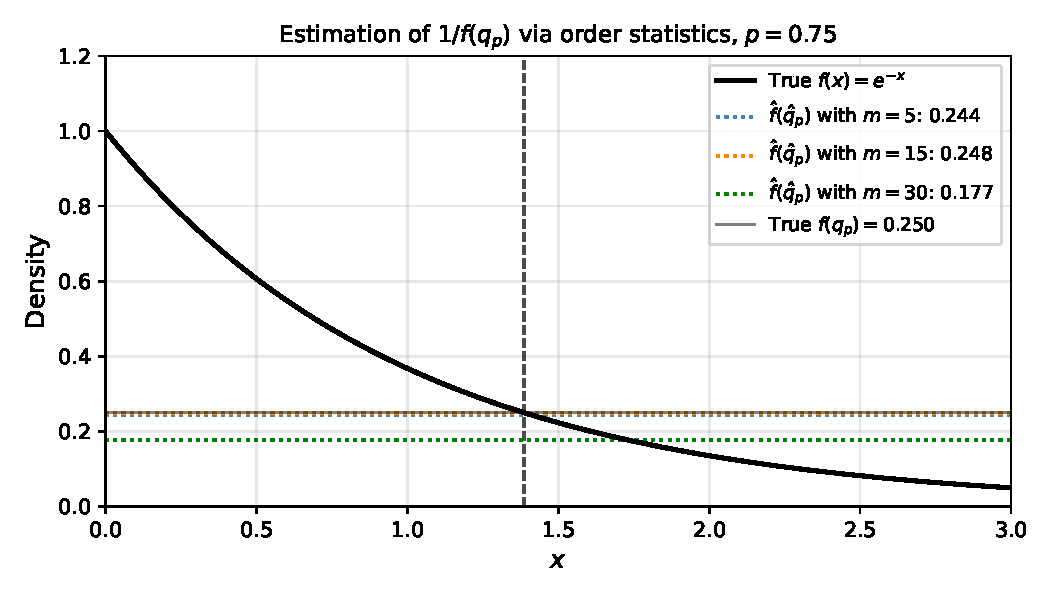
\includegraphics[width=0.60\textwidth]{fig_kde_quantile}
\end{center}

\end{frame}

\begin{frame}[fragile]{4.3 Python: Sample Quantile and Confidence Interval}
\begin{lstlisting}[style=python]
import numpy as np
from scipy import stats

def quantile_ci(X_samples, p, m=None, alpha=0.05):
    """
    Estimate the p-quantile and compute a confidence interval.
    X_samples : 1D array of i.i.d. samples from F
    p         : quantile level in (0, 1)
    m         : bandwidth (default: floor(sqrt(R)))
    """
    R        = len(X_samples)
    X_sorted = np.sort(X_samples)
    idx      = int(np.floor(p * R))     # index of sample quantile (0-based)
    q_hat    = X_sorted[idx]            # sample quantile

    if m is None:
        m = max(1, int(np.floor(np.sqrt(R))))  # simple bandwidth: sqrt(R)

    lo_idx = max(0, idx - m + 1)
    hi_idx = min(R - 1, idx + m)
    # Estimate 1/f(q_p) via finite difference of order statistics
    Q_prime_hat = R * (X_sorted[hi_idx] - X_sorted[lo_idx]) / (2 * m)

    z_q    = stats.norm.ppf(1 - alpha / 2)
    margin = z_q * np.sqrt(p * (1 - p) / R) * Q_prime_hat
    return q_hat, q_hat - margin, q_hat + margin

# Example: X ~ Exp(1), p=0.9, R=1000; true quantile = ln(10) ~ 2.3026
rng = np.random.default_rng(42)
X   = rng.exponential(1.0, size=1000)
q_hat, lo, hi = quantile_ci(X, p=0.9)
print(f"q_0.9 estimate: {q_hat:.4f}")
print(f"95% CI:         ({lo:.4f}, {hi:.4f})")
print(f"True q_0.9    = {np.log(10):.4f}")  # ln(10) ~ 2.3026
\end{lstlisting}
\end{frame}

%%==================================================================
%% SECTION 4.4 ABSOLUTE VS RELATIVE ERRORS
%%==================================================================

\begin{frame}[allowframebreaks]{4.4.1 The Chernoff Bound}

Section~4.4 studies absolute vs.\ relative errors more carefully, introducing
the \textbf{Chernoff bound} --- a powerful exponential concentration inequality.
Unlike Chebyshev's inequality (which gives polynomial decay $\sim 1/R$), the
Chernoff bound gives \emph{exponential decay} in $R$, making it enormously
sharper for large samples.

\begin{block}{Proposition~4.4.1 -- Chernoff Bound (Eqs.\ 4.1--4.3)}
  Let $S_R = Y_1 + \cdots + Y_R$ where $Y_i \overset{\text{i.i.d.}}{\sim} \mathrm{Bernoulli}(p)$
  (Bernoulli with parameter $p$: each $Y_i$ is 1 with probability $p$ and
  0 with probability $1-p$).  For any $0 < \varepsilon < 1$ (epsilon):
  \begin{align}
    \text{Upper tail:} & \quad
      \mathbb{P}(S_R \geq (1+\varepsilon)Rp)
        \leq \exp\!\left(-\frac{\varepsilon^2 Rp}{2+\varepsilon}\right)
        \leq \exp\!\left(-\frac{\varepsilon^2 Rp}{3}\right), \tag{4.1} \\[4pt]
    \text{Lower tail:} & \quad
      \mathbb{P}(S_R \leq (1-\varepsilon)Rp)
        \leq \exp\!\left(-\frac{\varepsilon^2 Rp}{2}\right). \tag{4.2}
  \end{align}
  Combining both tails (Eq.\ 4.3):
  \[
    \mathbb{P}(|S_R - Rp| \geq \varepsilon Rp) \leq 2\exp\!\left(-\frac{\varepsilon^2 Rp}{3}\right).
  \]
  Here $\exp(x)$ (exponential function) means $e^x$ where $e \approx 2.718$.
  Note that the bound decays \emph{exponentially} in $R$: it goes to zero
  much faster than any power of $R$.
\end{block}

\framebreak

\textbf{Proof sketch (exponential moment / Markov trick).}
For any $s > 0$, by Markov's inequality:
$\mathbb{P}(S_R \geq x) \leq e^{-sx}\mathbb{E}[e^{sS_R}]$.
For Bernoulli$_p$ variables: $\mathbb{E}[e^{sS_R}] = (pe^s + 1-p)^R \leq e^{Rp(e^s - 1)}$
(using $1+t \leq e^t$).  Choosing $s = \ln(1+\varepsilon)$ and applying
$\ln(1+\varepsilon) \geq \varepsilon^2/(2+\varepsilon)$ yields (4.1).

\begin{block}{Corollary~4.4.2 -- Required Replications for Relative Error (Eq.\ 4.4)}
  For $\hat{Y}_R = \frac{1}{R}\sum_{i=1}^R Y_i$ with $Y_i \sim \mathrm{Bernoulli}(p)$,
  and $\varepsilon, \delta \in (0,1)$: if
  \[
    R \geq \frac{3\ln(2/\delta)}{\varepsilon^2 p},
  \]
  then $\mathbb{P}(|\hat{Y}_R - p| \geq \varepsilon p) \leq \delta$.
  This controls \emph{relative} error at level $\varepsilon$.  Notice the
  critical $1/p$ factor: as $p \to 0$ (rare event), $R \to \infty$ proportionally.
\end{block}

\begin{exampleblock}{Example~4.4.3 -- Three Bounds for Bernoulli$(1/2)$, $\varepsilon = 1/2$}
  Compare $\mathbb{P}(|B_1 + \cdots + B_R - R/2| \geq R/4)$ under three bounds:
  \begin{itemize}
    \item \textbf{Chebyshev} (Eq.\ 4.5): $\leq 4/R$.  Polynomial decay.
    \item \textbf{Chernoff} (Eq.\ 4.6): $\leq 2e^{-R/24}$.  Exponential decay.
    \item \textbf{CLT approximation} (Eq.\ 4.7): $\approx \sqrt{8/(\pi R)}\,e^{-R/8}$.
      Sharpest, also exponential.
  \end{itemize}
  For $R = 1{,}000$: Chebyshev gives $0.004$; Chernoff gives
  $2e^{-41.7} \approx 1.7 \times 10^{-18}$; CLT gives $\approx 9 \times 10^{-55}$.
  The differences are astronomically large.
\end{exampleblock}

\begin{center}
  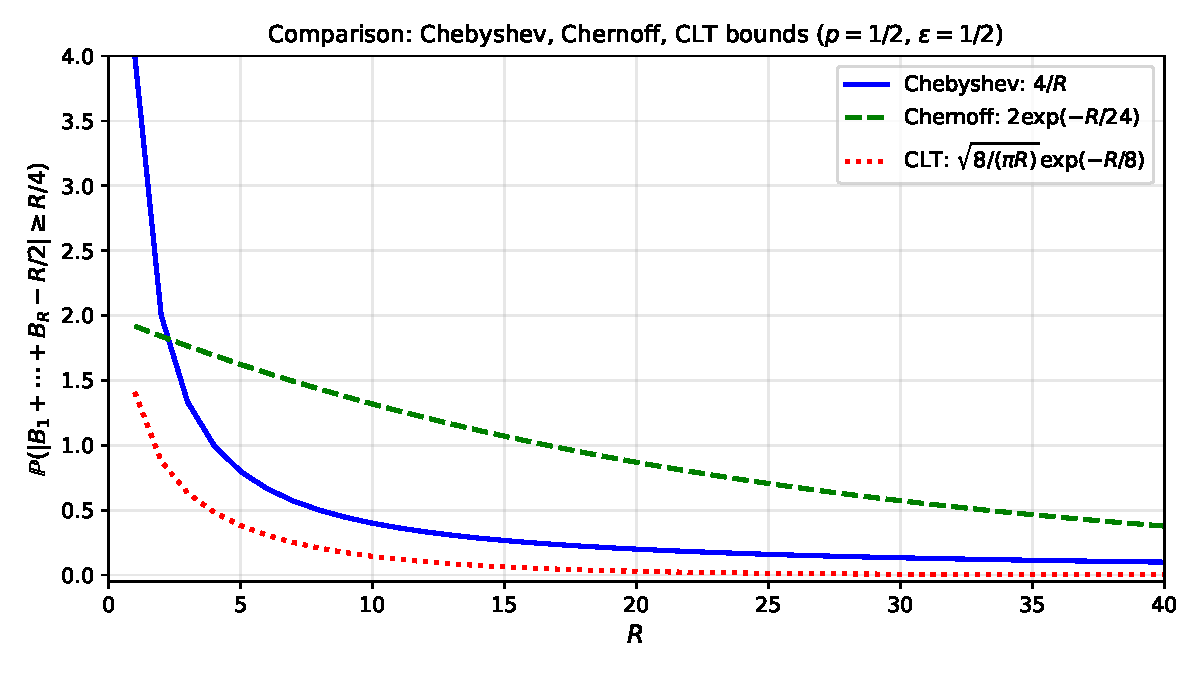
\includegraphics[width=0.60\textwidth]{fig_chernoff_comparison}
\end{center}

\end{frame}

\begin{frame}[allowframebreaks]{4.4.2 Discussion on Absolute vs Relative Errors}

Consider i.i.d.\ Bernoulli$(p)$ variables $Y_i$ with $I = p$, and fix
$\varepsilon = \delta = 0.01$.  The contrast between absolute and relative
error requirements is striking.

\textbf{Absolute error first.}  From the CLT formula (1.7) with
$\mathrm{Var}(Y) = p(1-p)$:
\[
  R^{\mathrm{abs}} = z_{1-\delta/2}^2 \frac{p(1-p)}{\varepsilon^2}
    = 2.576^2 \cdot \frac{p(1-p)}{0.01^2}.
\]
\begin{center}
  \begin{tabular}{ccc}
    \toprule
    $p = I$ & $\mathrm{Var}(Y) = p(1-p)$ & Required $R^{\mathrm{abs}}$ \\
    \midrule
    $0.1$ & $0.09$ & $\approx 5{,}945$ \\
    $0.01$ & $0.0099$ & $\approx 654$ \\
    $0.001$ & $\approx 0.001$ & $\approx 66$ \\
    \bottomrule
  \end{tabular}
\end{center}

Counterintuitively, \emph{smaller} $p$ requires \emph{fewer} replications for
absolute error control!  The reason: $\mathrm{Var}(Y) = p(1-p) \to 0$ as
$p \to 0$.  In the extreme: with $R=1$, $\hat{Y}_1 \in \{0,1\}$, and
$\mathbb{P}(|\hat{Y}_1 - p| \leq 0.01) = 1-p \geq 0.99$ for $p \leq 0.01$ ---
technically satisfies (E1) even though the estimate is essentially useless!

The absolute error condition is \emph{misleading} for rare events: the estimate
is usually 0 (which is ``close'' to $p$ in absolute terms when $p$ is tiny).

\framebreak

\textbf{Relative error corrects this flaw.}
From Corollary~4.4.2, to control $\mathbb{P}(|\hat{Y}_R - p| \geq \varepsilon p) \leq \delta$:
\[
  R \geq \frac{3\ln(2/\delta)}{\varepsilon^2 p}.
\]
\begin{center}
  \begin{tabular}{cc}
    \toprule
    $p = I$ & Required $R$ (Chernoff, $\varepsilon=\delta=0.01$) \\
    \midrule
    $0.1$ & $\approx 1.59 \times 10^6$ \\
    $0.01$ & $\approx 1.59 \times 10^7$ \\
    $0.001$ & $\approx 1.59 \times 10^8$ \\
    $10^{-6}$ & $\approx 1.59 \times 10^{11}$ \\
    \bottomrule
  \end{tabular}
\end{center}

Now $R \propto 1/p$: the required sample size grows \emph{inversely} with the
event probability.  For $p = 10^{-6}$, one would need about $10^{11}$
replications --- completely infeasible for naive Monte Carlo.

\begin{alertblock}{Key Insight: Rare Events Require Variance Reduction}
  Controlling relative error for small $I$ requires $R \propto 1/I$ replications.
  This is the fundamental hardness of rare-event simulation.  Variance reduction
  techniques such as importance sampling (Chapter~5) replace the standard estimator
  $Y$ with a lower-variance one, directly reducing the required $R$.  Without
  variance reduction, naive Monte Carlo is hopeless for rare events.
\end{alertblock}

\end{frame}

\begin{frame}[allowframebreaks]{4.4.3 Absolute vs Relative Error for Estimating $\pi$ (pi)}

Since $\pi \approx 3.14159$ is neither too small nor too large, both error
criteria lead to manageable sample sizes.  Using the hit-or-miss estimator
(Example~4.1.6): $Y_j = 4\mathbf{1}(U_{2j-1}^2+U_{2j}^2 \leq 1)$,
$\mathbb{E}Y = \pi$, $\mathrm{Var}(Y) \approx 2.697$.

Fix $\varepsilon = \delta = 0.01$ (i.e.\ $z_{1-\delta/2} = z_{0.995} = 2.576$).

\begin{block}{Absolute Error via CLT (Eq.\ 1.7)}
  \[
    R^{\mathrm{abs}} = z_{1-\delta/2}^2 \frac{\mathrm{Var}(Y)}{\varepsilon^2}
      = 2.576^2 \cdot \frac{2.697}{0.01^2} \approx 1.78 \times 10^5.
  \]
\end{block}

\begin{block}{Relative Error via Chernoff (Eq.\ 4.4)}
  For 1\% relative accuracy using the indicator $Y' = \mathbf{1}(U_1^2+U_2^2\leq 1)$
  with $\mathbb{E}Y' = \pi/4$:
  \[
    R^{\mathrm{rel,1}} \geq \frac{3\ln(2/0.01)}{0.01^2 \cdot (\pi/4)}
      = \frac{3 \times 5.298}{0.0001 \times 0.785} \approx 2.03 \times 10^5.
  \]
\end{block}

\begin{block}{Relative Error via CLT (comparing $\varepsilon' = 0.01/\pi$ absolute)}
  Setting the absolute tolerance to match 1\% relative:
  $\varepsilon' = 0.01\pi/\pi = 0.01$, and using the CLT:
  \[
    R^{\mathrm{rel,2}} = z_{1-\delta/2}^2 \frac{\mathrm{Var}(Y)}{\varepsilon^2 \pi^2}
      = 2.576^2 \cdot \frac{2.697}{0.01^2 \cdot \pi^2} \approx 5 \times 10^5.
  \]
\end{block}

Since $\pi \approx 3.14$ is not small, relative error is only $\sim 3\times$
harder than absolute error.  This is in stark contrast to rare events where
relative error is orders of magnitude harder.

\begin{center}
  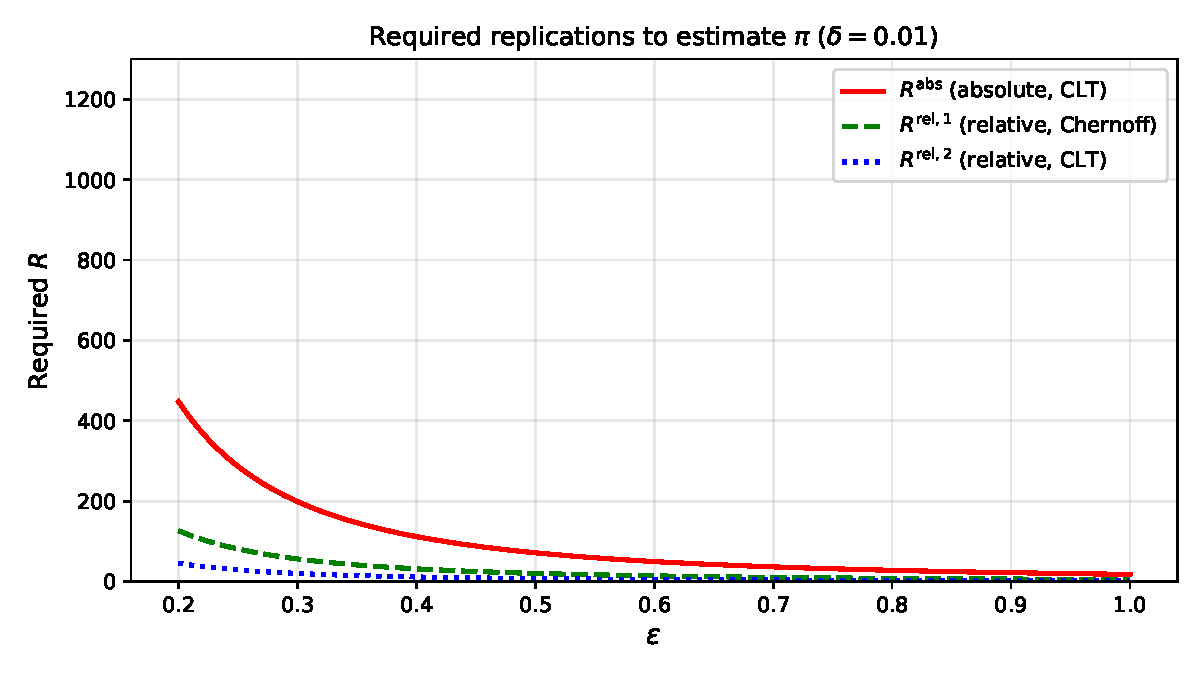
\includegraphics[width=0.60\textwidth]{fig_required_R_pi}
\end{center}

\end{frame}

\begin{frame}[allowframebreaks]{4.4.4 Influence of Variance on Absolute and Relative Errors}

The variance $\mathrm{Var}(\hat{I})$ of the estimator plays a fundamental role
in controlling both types of errors.  By the CLT, for large $R$,
the estimator is approximately $\hat{I} \sim \mathcal{N}(I, \mathrm{Var}(Y)/R)$.

\begin{block}{Required Replications: Summary Comparison}
  \begin{center}
  \begin{tabular}{lcc}
    \toprule
    Error type & Required $R$ & Grows as \\
    \midrule
    Absolute ($|\hat{I} - I| \leq \varepsilon$) &
      $R = z_{1-\delta/2}^2\,\mathrm{Var}(Y)/\varepsilon^2$ &
      $\propto 1/\varepsilon^2$ \\[4pt]
    Relative ($|\hat{I}/I - 1| \leq \varepsilon$) &
      $R = z_{1-\delta/2}^2\,\mathrm{Var}(Y)/(\varepsilon^2 I^2)$ &
      $\propto 1/(\varepsilon^2 I^2)$ \\
    \bottomrule
  \end{tabular}
  \end{center}
  The relative error formula has an extra $1/I^2$ factor.  When $I$ is small,
  this creates an enormous gap between the two requirements.
\end{block}

\textbf{Key message:} Reducing $\mathrm{Var}(Y)$ benefits both error criteria:
for absolute error, it reduces $R$ proportionally; for relative error (when
$I$ is small), reducing $\mathrm{Var}(Y)$ by a factor of $c$ reduces the
required $R$ by the same factor $c$.  This underscores why variance reduction
techniques of Chapter~5 (importance sampling, stratification, control variates)
are essential for rare-event simulation.

\end{frame}

\begin{frame}[fragile]{4.4 Python: Comparing Error Bounds}
\begin{lstlisting}[style=python]
import numpy as np
from scipy import stats

def R_absolute_clt(sigma2, epsilon, delta):
    """Required R for absolute error control via CLT."""
    z = stats.norm.ppf(1 - delta / 2)
    return z**2 * sigma2 / epsilon**2

def R_relative_chernoff(p, epsilon, delta):
    """Required R for relative error via Chernoff (Bernoulli p only)."""
    return 3 * np.log(2 / delta) / (epsilon**2 * p)

def R_relative_clt(sigma2, I, epsilon, delta):
    """Required R for relative error via CLT (any distribution)."""
    z = stats.norm.ppf(1 - delta / 2)
    return z**2 * sigma2 / (epsilon**2 * I**2)

# Hit-or-miss estimator for pi
VarY = 16 * (np.pi / 4) * (1 - np.pi / 4)  # ~ 2.697
I    = np.pi
eps  = 0.01
delt = 0.01

R_abs  = R_absolute_clt(VarY, eps, delt)
R_rel1 = R_relative_chernoff(np.pi / 4, eps, delt)  # on indicator Y'=1(hit)
R_rel2 = R_relative_clt(VarY, I, eps, delt)

print(f"R_abs  (absolute, CLT):       {R_abs:.2e}")   # ~1.78e+05
print(f"R_rel1 (relative, Chernoff):  {R_rel1:.2e}")  # ~2.03e+05
print(f"R_rel2 (relative, CLT):       {R_rel2:.2e}")  # ~5.0e+05
\end{lstlisting}
\end{frame}

%%==================================================================
%% SECTION 4.5 CONCLUSIONS
%%==================================================================

\begin{frame}[allowframebreaks]{4.5 Conclusions: The Fundamental Relationship Revisited}

The core result of Chapter~4 is the \textbf{fundamental relationship} that
governs the accuracy of all Monte Carlo estimators based on independent
replications.  Regardless of the specific estimation problem (mean, transformed
mean, or quantile), the half-width of the confidence interval has the form:

\begin{block}{The Fundamental Relationship (Eq.\ 5.1)}
  \[
    b = \frac{z_{1-\alpha/2}\,D}{\sqrt{R}},
  \]
  where $b$ is the CI half-width, $R$ is the number of replications,
  $z_{1-\alpha/2}$ is the normal quantile (for 95\%: $z_{0.975} = 1.96$),
  and $D$ is the variability constant depending on the problem:
  \begin{itemize}
    \item Estimating $I = \mathbb{E}Y$ (one-dimensional):\quad
      $D = \sigma_Y = \sqrt{\mathrm{Var}(Y)}$.
    \item Estimating $z = k(I)$ with $I = \mathbb{E}Y$: \quad
      $D = |k'(I)|\,\sigma_Y$.
    \item Estimating $z = k(\mathbf{I})$ with $\mathbf{I} = \mathbb{E}\mathbf{Y}$ (multi-D):
      \quad $D = \sqrt{\nabla k(\mathbf{I})\,\boldsymbol{\Sigma}_{\mathbf{Y}}\,(\nabla k(\mathbf{I}))^T}$.
    \item Estimating quantile $q_p$:\quad
      $D = \sqrt{p(1-p)}/f(q_p)$.
  \end{itemize}
  In all cases the error decreases at the \emph{Monte Carlo rate} $O(R^{-1/2})$,
  \textbf{independent of dimension $d$}.
\end{block}

\framebreak

\textbf{Practical workflow for a Monte Carlo study:}
\begin{enumerate}
  \item Run a \emph{pilot simulation} of size $m$ to estimate $D$
    (equivalently, $\sigma_Y^2$ or $\boldsymbol{\Sigma}_{\mathbf{Y}}$).
  \item Compute the required $R = z_{1-\alpha/2}^2 D^2/b^2$ for the desired
    half-width $b$ and confidence level $1-\alpha$.
  \item Run $R$ main replications; compute estimates and sample statistics.
  \item Report the point estimate and confidence interval.
\end{enumerate}

\begin{block}{Summary of Confidence Intervals (for $\alpha = 0.05$, $z_{0.975} = 1.96$)}
  \begin{center}\small
    \begin{tabular}{lll}
      \toprule
      Quantity & Point Estimate & 95\% CI \\
      \midrule
      $I = \mathbb{E}Y$
        & $\hat{Y}_R$
        & $\hat{Y}_R \pm \dfrac{1.96\,\hat{S}_R}{\sqrt{R}}$ \\[8pt]
      $k(I)$, $I = \mathbb{E}Y$
        & $k(\hat{Y}_R)$
        & $k(\hat{Y}_R) \pm \dfrac{1.96\,\hat{S}_R\,|k'(\hat{Y}_R)|}{\sqrt{R}}$ \\[8pt]
      $k(\mathbf{I})$, $\mathbf{I} = \mathbb{E}\mathbf{Y}$
        & $k(\hat{\mathbf{Y}}_R)$
        & $k(\hat{\mathbf{Y}}_R) \pm 1.96\,\dfrac{\hat{\varsigma}}{\sqrt{R}}$ \\[8pt]
      $q_p$ (quantile)
        & $X_{(\lfloor pR\rfloor)}$
        & $\hat{q}_p \pm 1.96\sqrt{\dfrac{p(1-p)}{R}}\,\hat{Q}'_{p,R}$ \\
      \bottomrule
    \end{tabular}
  \end{center}
\end{block}

\framebreak

\begin{alertblock}{Key Takeaways of Chapter 4}
  \begin{itemize}
    \item The Monte Carlo rate $b = O(R^{-1/2})$ holds in \emph{any} dimension:
      there is \textbf{no curse of dimensionality} for the statistical error.
    \item The CLT-based formula requires only $\approx 19\%$ as many replications
      as the (valid but conservative) Chebyshev bound.
    \item Transformed estimators $k(\hat{Y}_R)$ are generally biased with bias
      $O(R^{-1})$, dominated by std dev $O(R^{-1/2})$ for large $R$; bias
      corrections are usually unnecessary.
    \item \textbf{Relative error} is far harder than absolute error when $I$ is small;
      required $R \propto 1/I$ making naive MC infeasible for rare events.
      Variance reduction (Chapter~5) is essential.
    \item For quantile estimation: $\varsigma^2 = p(1-p)/f(q_p)^2$ -- the density
      at the quantile must be estimated via order statistics, with bandwidth
      $m_R \sim \sqrt{R}$ (simple) or $m_R \sim R^{4/5}$ (MSE-optimal).
    \item Three shapes of confidence regions for multivariate means trade off
      tightness (ellipsoid, smallest) vs.\ computational ease (rectangle, largest).
  \end{itemize}
\end{alertblock}

\end{frame}

\begin{frame}[fragile]{4.5 Python: Full Output Analysis Workflow}
\begin{lstlisting}[style=python]
import numpy as np
from scipy import stats

def full_mc_analysis(simulate_Y, R_pilot=500, b=0.05, alpha=0.05, seed=42):
    """Complete Monte Carlo output analysis pipeline."""
    rng = np.random.default_rng(seed)

    # Step 1: Pilot simulation to estimate Var(Y)
    Y_pilot    = np.array([simulate_Y(rng) for _ in range(R_pilot)])
    sigma2_hat = Y_pilot.var(ddof=1)
    print(f"Pilot sigma^2 estimate: {sigma2_hat:.4f}")

    # Step 2: Required R from the fundamental relationship b = z * sigma / sqrt(R)
    z      = stats.norm.ppf(1 - alpha / 2)
    R_main = int(np.ceil(z**2 * sigma2_hat / b**2))
    print(f"Required R (b={b}, alpha={alpha}): {R_main}")

    # Step 3: Main simulation
    Y_main = np.array([simulate_Y(rng) for _ in range(R_main)])
    Y_bar  = Y_main.mean()
    S      = Y_main.std(ddof=1)

    ci_lo = Y_bar - z * S / np.sqrt(R_main)
    ci_hi = Y_bar + z * S / np.sqrt(R_main)
    print(f"Estimate: {Y_bar:.4f}")
    print(f"95% CI  : ({ci_lo:.4f}, {ci_hi:.4f})")
    return Y_bar, (ci_lo, ci_hi)

# Estimate pi using hit-or-miss estimator; E[Y] = pi, Var(Y) ~ 2.697
def sim_pi(rng):
    u = rng.random(2)
    return 4.0 * float(u[0]**2 + u[1]**2 <= 1)

est, ci = full_mc_analysis(sim_pi, R_pilot=1000, b=0.05)
print(f"True pi = {np.pi:.4f}")
\end{lstlisting}
\end{frame}

%% ---- Final summary slide
\begin{frame}{Chapter 4: Summary}
  \begin{columns}
    \begin{column}{0.48\textwidth}
      \textbf{Section 4.1 -- Estimating $I = \mathbb{E}Y$:}
      \begin{itemize}\small
        \item Sample mean $\hat{Y}_R$: unbiased, strongly consistent
        \item Chebyshev: $b_R = \sigma_Y/(\alpha^{1/2}\sqrt{R})$ (valid, loose)
        \item CLT: $b = z_{1-\alpha/2}\sigma_Y/\sqrt{R}$ (sharp, asymptotic)
        \item Required $R = z_{1-\alpha/2}^2\sigma_Y^2/b^2$
        \item CLT needs only $\approx 19\%$ of Chebyshev's $R$
        \item Online updates (Eqs.\ 1.11--1.12) for streaming computation
        \item Multivariate: ellipsoid, parallelogram, rectangle regions
      \end{itemize}
      \medskip
      \textbf{Section 4.2 -- Estimating $k(I)$:}
      \begin{itemize}\small
        \item Delta method: $\varsigma^2 = k'(I)^2\sigma_Y^2$
        \item Multi-D: $\varsigma^2 = \nabla k(\mathbf{I})\boldsymbol{\Sigma}(\nabla k)^T$
        \item Bias $O(R^{-1})$ negligible vs std dev $O(R^{-1/2})$
        \item MSE = Variance + Bias$^2$; bias usually negligible
      \end{itemize}
    \end{column}
    \begin{column}{0.50\textwidth}
      \textbf{Section 4.3 -- Quantile estimation:}
      \begin{itemize}\small
        \item $\hat{q}_p = X_{(\lfloor pR\rfloor)}$: consistent, CLT holds
        \item Asymptotic variance: $\varsigma^2 = p(1-p)/f(q_p)^2$
        \item Estimate $1/f(q_p)$ via order-stat finite differences
        \item Bandwidth: $m_R \sim \sqrt{R}$ (simple) or $m_R \sim R^{4/5}$ (optimal)
      \end{itemize}
      \medskip
      \textbf{Section 4.4 -- Error bounds:}
      \begin{itemize}\small
        \item Chernoff: exponential bound (vs polynomial Chebyshev)
        \item Absolute: $R \propto \mathrm{Var}(Y)/\varepsilon^2$
        \item Relative: $R \propto \mathrm{Var}(Y)/(\varepsilon^2 I^2)$
        \item Rare events ($I \ll 1$): $R \propto 1/I$ -- need variance reduction
      \end{itemize}
      \medskip
      \begin{center}
        \begin{alertblock}{}
          \centering
          \textbf{Monte Carlo rate: $b = O(R^{-1/2})$}\\
          \small dimension-independent
        \end{alertblock}
      \end{center}
    \end{column}
  \end{columns}
\end{frame}

\end{document}
